\documentclass[10pt]{article}
\usepackage{tmlr}

\usepackage{amsmath,amssymb,amsfonts,amsthm,bm,mathtools}
\usepackage{booktabs}
\usepackage{multirow}
\usepackage{xcolor}
\usepackage{graphicx}
\usepackage{microtype}
\usepackage{url}
\usepackage{hyperref}

\hypersetup{
    colorlinks=true,
    linkcolor=blue!60!black,
    citecolor=blue!60!black,
    urlcolor=blue!60!black
}

\newtheorem{theorem}{Theorem}
\newtheorem{proposition}{Proposition}
\newtheorem{lemma}{Lemma}
\newtheorem{corollary}{Corollary}
\theoremstyle{definition}
\newtheorem{definition}{Definition}
\newtheorem{assumption}{Assumption}
\theoremstyle{remark}
\newtheorem{remark}{Remark}

\newcommand{\R}{\mathbb{R}}
\newcommand{\Sp}{\mathbb{S}}
\newcommand{\Tor}{\mathbb{T}}
\newcommand{\norm}[1]{\left\lVert #1 \right\rVert}
\newcommand{\abs}[1]{\left\lvert #1 \right\rvert}
\newcommand{\inner}[1]{\left\langle #1 \right\rangle}
\DeclareMathOperator{\rank}{rank}
\DeclareMathOperator{\diag}{diag}
\DeclareMathOperator{\Var}{Var}
\DeclareMathOperator{\CV}{CV}
\DeclareMathOperator{\OVR}{OVR}

\title{Conditional Radial Foliation in Norm-Preserving Dynamical Autoencoders}

\begin{document}

\maketitle

\begin{abstract}
Under exact intertwining, a norm-preserving latent transition makes the encoder norm a conserved quantity, but this alone does not identify the physical invariants. We characterize when it does. Under exact intertwining, regular level sets, and dense sampled orbits on a dense set of invariant values, the latent radius is constant on every level set. If the encoder is globally injective, the latent and observed dimensions match, and the level sets are compact and connected, the radius is a continuous strictly monotone coordinate for a scalar invariant. We also establish two limitations: disjoint enclosed basins cannot both map to origin-centered spheres under an injective encoder, and one continuous scalar radius cannot identify an open set of multiple independent invariants. For compact toroidal leaves, preserving a radius in each of $K$ planar latent blocks instead identifies the invariant vector up to a homeomorphism. These conditional results use standard separation and invariance-of-domain arguments. Supporting analysis distinguishes exact radial gradient pullback from forward dynamical isometry and treats stabilized normalization explicitly. Experiments on discrete nonlinear Schr\"odinger dynamics, Lotka--Volterra dynamics, and coupled oscillators examine conservation, prediction, and invariant readout separately, including controls for resonance and encoder translation. A two-block ablation shows that the strongest empirical recovery also relies on a radius-dependent frequency prior in our fixed training protocol.
\end{abstract}

\section{Introduction}
\label{sec:intro}

Norm-preserving latent dynamics provide a simple architectural prior for conservative systems. Given an encoder $E$, a latent transition $g$ with $\norm{g(z)}_2=\norm{z}_2$, and exact intertwining $E\circ\Phi_{\Delta t}=g\circ E$, the quantity $h(x)=\norm{E(x)}_2$ is invariant under the observed time-step map. This fact leaves an identification question: when does $h$ distinguish physical invariant levels, and when can it remain uninformative despite accurate dynamics? We address this question through the geometry of the level sets and the injectivity of the encoder.

The normalization primitive studied here transfers the input magnitude to a transformed direction:
\begin{equation}
    \operatorname{SkipNorm}_p(x; f) \coloneqq \frac{f(x)}{\norm{f(x)}_p} \norm{x}_p, \qquad x \ne 0,\quad f(x)\ne0.
    \label{eq:skipnorm_def}
\end{equation}
For $p=2$, projecting a residual branch onto the input sphere's tangent space before normalization gives the spherical retraction we call Geodesic SkipNorm. This geometric update is established in manifold optimization \citep{absil2008optimization}; SpheretNorm uses the same projection--retraction and derives its radial pullback identity \citep{zhang2026spheretnorm}. Our contribution is the conditional identification theory for dynamical autoencoders, rather than priority for this update.

Norm preservation and dynamical isometry are different properties. The exact identity $J^\top u_{\mathrm{out}}=u_{\mathrm{in}}$ holds for every differentiable Euclidean norm-preserving map away from zero, including maps between different dimensions. A forward radial singular pair exists precisely when radial perturbations produce no angular change; other unit singular values may exist without this condition. We give the general Jacobian decomposition and exact rank condition. For comparison, ideal gain-free RMSNorm removes radial scale and ideal LayerNorm also removes the mean, whereas positive stabilizers retain radial sensitivity and learned affine parameters change the primitive spectra \citep{ba2016layer, zhang2019root}. These distinctions matter when interpreting gradient and conservation measurements.

Our main results concern regular invariant level sets. Density of a sampled orbit makes any continuous invariant constant on its closure. Combined with global encoder injectivity and matched dimensions, invariance of domain then forces a compact connected scalar level set to fill an entire latent sphere, making its radius a strictly monotone invariant coordinate. For multiple invariants, $K$ planar norm-preserving blocks provide the corresponding product of circles. The hypotheses are substantive: disconnected basins obstruct a common spherical representation, and resonant orbits need not explore an entire level set. Approximate training does not by itself certify injectivity or exact intertwining.

\paragraph{Contributions.}
\begin{enumerate}
    \item We state and prove scalar and toroidal radial-foliation theorems, allowing sampled-orbit density on a dense set of regular invariant values, and identify the dimension and injectivity conditions needed for invariant recovery (Sections~\ref{sec:foliation} and \ref{sec:torus}).
    \item We establish the obstruction for disjoint enclosed basins and give resonance and translation controls that delimit what radial constancy and relative errors can establish (Section~\ref{sec:obstructions}).
    \item We derive the rectangular Jacobian and rank formulas and stabilized primitive normalization spectra, then evaluate norm preservation, trajectory error, and invariant readout as distinct outcomes (Sections~\ref{sec:geometry}--\ref{sec:torus}).
\end{enumerate}

\section{Related Work}
\label{sec:related}

\paragraph{Normalization and spherical updates.}
Without affine parameters or stabilizers, LayerNorm maps centered activations onto a sphere in the zero-mean hyperplane, while RMSNorm fixes the Euclidean radius \citep{ba2016layer, zhang2019root}. These are statements about the primitive operators, not arbitrary pre-normalized residual blocks. Weight Normalization separates magnitude and direction in parameter space \citep{salimans2016weight}, and hyperspherical VAEs use directional latent distributions \citep{davidson2018hyperspherical, xu2018spherical}. nGPT normalizes hidden states and updates on the sphere \citep{loshchilov2024ngpt}; GeoNorm projects updates into the tangent space and uses a spherical exponential map \citep{zheng2026geonorm}. SpheretNorm's projection--retraction update coincides with the tangent-projected norm-preserving update analyzed here, and its Appendix~D.7 gives the corresponding radial pullback identity \citep{zhang2026spheretnorm}. We use this established primitive to study conditions for latent invariant identification.

\paragraph{Orthogonal transitions and dynamical isometry.}
Dynamical isometry concerns the full singular spectrum of a network Jacobian \citep{saxe2014exact, pennington2017resurrecting}; preserving a state norm alone does not ensure it. Orthogonal and unitary recurrent models use structured products, exponential maps, and Cayley transforms \citep{arjovsky2016unitary, lezcano2019cheap, helfrich2018orthogonal}. Tall linear isometries can also preserve norms across a dimension increase. State-dependent orthogonal maps need not all incur cubic cost: our timing comparison concerns the dense Cayley implementation, which solves a dense linear system at each step. The spherical retraction itself uses $\mathcal{O}(d)$ arithmetic in addition to the cost of its learned vector field.

\paragraph{Conservation laws and latent dynamical representations.}
Hamiltonian Neural Networks and Symplectic ODE-Nets exploit Hamiltonian structure \citep{greydanus2019hamiltonian, zhong2020symplectic}; Lagrangian Neural Networks formulate dynamics through learned Lagrangians in configuration--velocity coordinates \citep{cranmer2020lagrangian}. Invariant-discovery approaches include Siamese invariant learning \citep{wetzel2020discovering} and trajectory manifold learning \citep{liu2021ai}, learned first integrals with projected dynamics in COMET \citep{otto2023learning}, and contrastively learned invariant representations with a dynamics projection layer in ConCerNet \citep{zhang2023concernet}. Learned latent dynamical coordinates also connect to Koopman autoencoders \citep{lusch2018deep}. Our results characterize what a particular architectural invariant---the latent norm or vector of block norms---identifies under exact intertwining. The proofs apply standard topological tools \citep{brouwer1911beweis, hatcher2002algebraic}; they do not guarantee that finite-data optimization satisfies their hypotheses or that the recovered coordinates are canonical actions.

\section{Differential Geometry of SkipNorm and Stabilized Normalizers}
\label{sec:geometry}

We first analyze the exact first-order differential geometry of SkipNorm, compare its Jacobian spectrum against $\varepsilon$-stabilized RMSNorm and LayerNorm, and introduce tangent-projected Geodesic SkipNorm. All proofs and explicit counterexample derivations are provided in Appendix~\ref{app:geometry_proofs}.

\subsection{Exact Jacobian Decomposition and Cotangent Radial Pullback}

Let $x \in \R^{d_{\mathrm{in}}} \setminus \{0\}$ with radius $r = \norm{x}_2 > 0$ and unit radial direction $u_{\mathrm{in}} = x / r \in \Sp^{d_{\mathrm{in}}-1}$. Let $f: \R^{d_{\mathrm{in}}} \to \R^{d_{\mathrm{out}}}$ be $C^1$ on a neighborhood of $x$ with $y = f(x) \neq 0$, output unit direction $u_{\mathrm{out}} = y / \norm{y}_2 \in \Sp^{d_{\mathrm{out}}-1}$, and unstabilized Euclidean SkipNorm map
\begin{equation}
    F(x) \coloneqq \frac{f(x)}{\norm{f(x)}_2} \norm{x}_2 = r \, u_{\mathrm{out}}(x), \qquad \norm{F(x)}_2 = \norm{x}_2.
    \label{eq:skipnorm_l2}
\end{equation}
A possible stabilized implementation is $F_\varepsilon(x) = f(x) \sqrt{\norm{x}_2^2 + \varepsilon} / \sqrt{\norm{f(x)}_2^2 + \varepsilon}$. It does not preserve the norm exactly in general; all identities below refer to the ideal map $F$ on its nonzero domain. Differentiating $\norm{u_{\mathrm{out}}(x)}_2^2 \equiv 1$ gives $u_{\mathrm{out}}^\top D_x u_{\mathrm{out}}(x) = 0$, so the image of $D_x u_{\mathrm{out}}(x) = \norm{y}_2^{-1}(I_{d_{\mathrm{out}}} - u_{\mathrm{out}} u_{\mathrm{out}}^\top) D_x f(x)$ lies strictly in the tangent hyperplane $T_{u_{\mathrm{out}}} \Sp^{d_{\mathrm{out}}-1} = u_{\mathrm{out}}^\perp$. Decomposing $\R^{d_{\mathrm{in}}} = \operatorname{span}(u_{\mathrm{in}}) \oplus u_{\mathrm{in}}^\perp$ and $\R^{d_{\mathrm{out}}} = \operatorname{span}(u_{\mathrm{out}}) \oplus u_{\mathrm{out}}^\perp$ reveals the exact structure of the Jacobian $J(x) = D_x F(x)$.

\begin{proposition}[Exact Jacobian Geometry of Euclidean SkipNorm]
\label{prop:skipnorm_jacobian}
Let $F$ be given by Eq.~\eqref{eq:skipnorm_l2} near $x\ne0$, with $f$ of class $C^1$ and $f(x)\ne0$. Define the radial-to-angular sensitivity vector $B(x) \in u_{\mathrm{out}}^\perp$ and the tangential-to-angular operator $A_{\perp}(x): u_{\mathrm{in}}^\perp \to u_{\mathrm{out}}^\perp$ by
\begin{equation}
    B(x) \coloneqq r (D_x u_{\mathrm{out}}(x)) u_{\mathrm{in}} = \left. r \frac{\partial u_{\mathrm{out}}(r u_{\mathrm{in}})}{\partial r} \right|_{r = \norm{x}_2} \in u_{\mathrm{out}}^\perp, \qquad A_{\perp}(x) \coloneqq \left. r D_x u_{\mathrm{out}}(x) \right|_{u_{\mathrm{in}}^\perp}.
    \label{eq:B_and_Aperp}
\end{equation}
Then:
\begin{enumerate}
    \item[\textbf{(a)}] \textbf{Full Jacobian and Block Matrix Representation:} In any orthonormal bases $\{u_{\mathrm{in}}, v_1, \dots, v_{d_{\mathrm{in}}-1}\}$ of $\R^{d_{\mathrm{in}}}$ and $\{u_{\mathrm{out}}, w_1, \dots, w_{d_{\mathrm{out}}-1}\}$ of $\R^{d_{\mathrm{out}}}$,
    \begin{equation}
        J(x) = u_{\mathrm{out}} u_{\mathrm{in}}^\top + B(x) u_{\mathrm{in}}^\top + A_{\perp}(x) P_{u_{\mathrm{in}}^\perp}, \qquad
        [J(x)] = \begin{pmatrix} 1 & 0_{1 \times (d_{\mathrm{in}}-1)} \\ b & \tilde{A} \end{pmatrix} \in \R^{d_{\mathrm{out}} \times d_{\mathrm{in}}},
        \label{eq:jacobian_block}
    \end{equation}
    where $b \in \R^{d_{\mathrm{out}}-1}$ and $\tilde{A} \in \R^{(d_{\mathrm{out}}-1)\times (d_{\mathrm{in}}-1)}$ represent $B(x)$ and $A_\perp(x)$.
    \item[\textbf{(b)}] \textbf{Unconditional Cotangent Radial Pullback:} Across all dimensions $d_{\mathrm{in}}, d_{\mathrm{out}} \ge 1$ and all $C^1$ branches $f$, the transpose Jacobian satisfies
    \begin{equation}
        J(x)^\top u_{\mathrm{out}} = u_{\mathrm{in}}, \qquad \norm{J(x)^\top u_{\mathrm{out}}}_2 = 1, \qquad \sigma_{\max}(J(x)) \ge 1.
        \label{eq:cotangent_pullback}
    \end{equation}
    Furthermore, for any composition $F_{\mathrm{total}} = F_L \circ \cdots \circ F_1$ of $L$ SkipNorm layers with $x_\ell = F_\ell(x_{\ell-1}) \neq 0$, the end-to-end Jacobian $J_{\mathrm{total}} = \prod_{\ell=1}^L J_\ell$ satisfies $J_{\mathrm{total}}^\top u_L = u_0$ and $\norm{J_{\mathrm{total}}^\top u_L}_2 = 1$ identically.
    \item[\textbf{(c)}] \textbf{Conditional Forward Pushforward and Unit Singular Value:} The forward radial pushforward equals $J(x) u_{\mathrm{in}} = u_{\mathrm{out}} + B(x)$ with $\norm{J(x) u_{\mathrm{in}}}_2 = \sqrt{1 + \norm{B(x)}_2^2}$. Consequently, $J(x) u_{\mathrm{in}} = u_{\mathrm{out}}$ if and only if $B(x) = 0$ (which holds automatically whenever $f$ is positively homogeneous of any degree $\gamma \in \R$, i.e., $f(\lambda x) = \lambda^\gamma f(x)$ for $\lambda > 0$). When $B(x) = 0$, the block matrix $[J(x)] = \diag(1, \tilde{A})$ decouples orthogonally, so $\sigma = 1$ is an exact singular value of $J(x)$ with left/right singular vectors $(u_{\mathrm{out}}, u_{\mathrm{in}})$ and the remaining singular values are $\sigma(\tilde{A})$. If $B(x)\ne0$, this radial singular pair is absent, although unrelated unit singular values can still occur.
    \item[\textbf{(d)}] \textbf{Explicit Counterexamples when $B(x) \neq 0$:}
    \begin{enumerate}
        \item[\emph{(i)}] \emph{Equidimensional Twist ($d_{\mathrm{in}} = d_{\mathrm{out}} = 2$):} For $f(x) = R_{\log \norm{x}_2} x$, where $R_\theta \in \mathrm{SO}(2)$ is planar rotation by $\theta = \log \norm{x}_2$, we have $\norm{f(x)}_2 = \norm{x}_2$ so $F(x) = f(x)$. At $x = e_1 = (1, 0)^\top$, $B(e_1) = e_2 \neq 0$ and
        \begin{equation*}
            J(e_1) = \begin{pmatrix} 1 & 0 \\ 1 & 1 \end{pmatrix}, \qquad \sigma(J(e_1)) = \left\{\varphi, \varphi^{-1}\right\} = \left\{\frac{\sqrt{5}+1}{2}, \frac{\sqrt{5}-1}{2}\right\} \approx \{1.6180, 0.6180\}.
        \end{equation*}
        Thus $1 \notin \sigma(J(e_1))$ even though $d_{\mathrm{in}} = d_{\mathrm{out}} = 2$ and $\norm{F(x)}_2 \equiv \norm{x}_2$.
        \item[\emph{(ii)}] \emph{Dimension-Changing Spiral ($d_{\mathrm{in}} = 1, d_{\mathrm{out}} = 2$):} For $x = t > 0$ and $f(t) = (\cos \log t, \sin \log t)^\top$, $F(t) = t (\cos \log t, \sin \log t)^\top$ satisfies $\norm{F(t)}_2 = t$. At $t = 1$, $J(1) = (1, 1)^\top$, whose sole singular value is $\sigma_1(J(1)) = \sqrt{2} \approx 1.4142 \neq 1$, while $J(1)^\top u_{\mathrm{out}} = 1 = u_{\mathrm{in}}$.
    \end{enumerate}
\end{enumerate}
\end{proposition}

Proposition~\ref{prop:skipnorm_jacobian} clarifies a critical geometric distinction: norm preservation $\norm{F(x)}_2 = \norm{x}_2$ is a statement on the \emph{cotangent bundle} ($d(\norm{F(x)}_2) = d(\norm{x}_2) \implies J(x)^\top u_{\mathrm{out}} = u_{\mathrm{in}}$), not on the forward pushforward $J(x) u_{\mathrm{in}}$. Whenever a nonlinear layer $f(x)$ alters its output direction as the input radius $r = \norm{x}_2$ varies ($B(x) \neq 0$), a radial perturbation $\delta x = \delta r \, u_{\mathrm{in}}$ induces both a radial step $\delta r \, u_{\mathrm{out}}$ and a tangential shear $\delta r \, B(x)$. Nevertheless, because the top row of $[J(x)]$ in Eq.~\eqref{eq:jacobian_block} is $(1, 0)$ regardless of $b$, backward propagation of radial gradients ($J(x)^\top u_{\mathrm{out}} = u_{\mathrm{in}}$) and the rank decoupling $\rank(J(x)) = 1 + \rank(\tilde{A})$ hold unconditionally.

\begin{figure}[t]
    \centering
    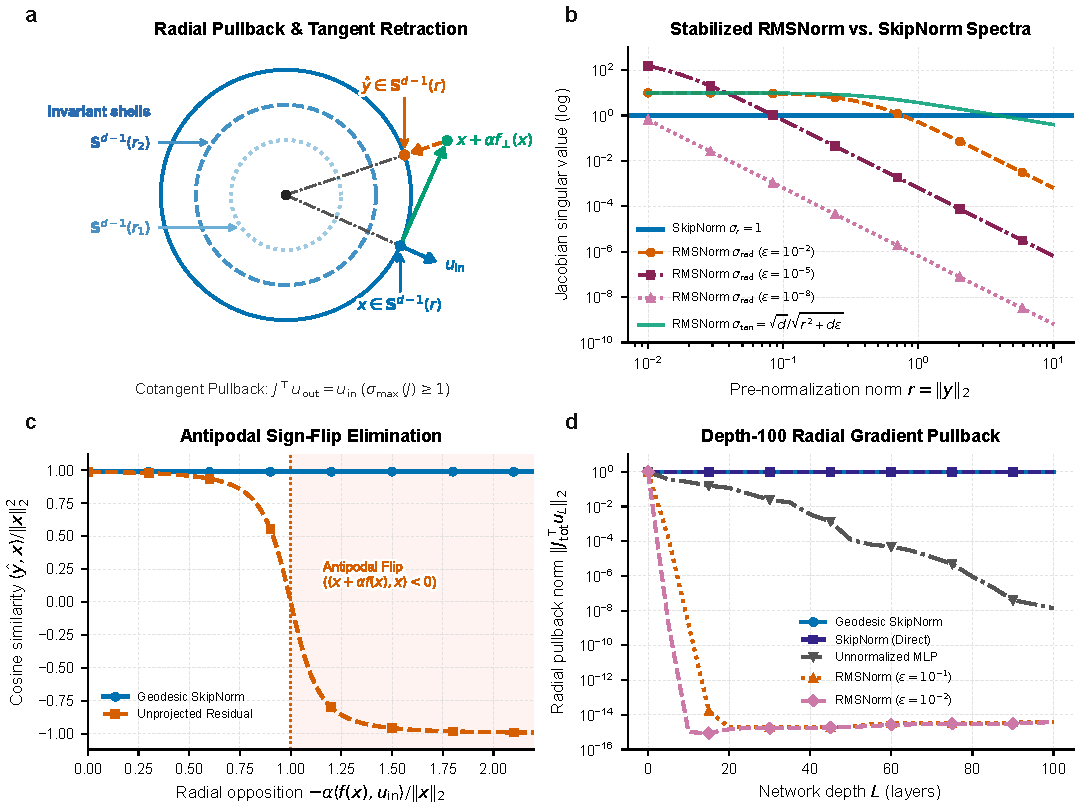
\includegraphics[width=\textwidth]{fig1_geometry_and_spectra.pdf}
    \caption{\textbf{Exact Jacobian geometry of SkipNorm, stabilized normalizer spectra, and tangent-space Geodesic retraction.}
    \textbf{(a)} Geometric decomposition on $\Sp^{d-1}(r)$: Geodesic SkipNorm projects $f(x)$ onto $T_x \Sp^{d-1}(r)$ before retracting onto the input sphere, guaranteeing the unconditional cotangent radial pullback $J^\top u_{\mathrm{out}} = u_{\mathrm{in}}$.
    \textbf{(b)} Exact singular values of $\varepsilon$-stabilized RMSNorm ($d=16$) versus pre-normalization norm $r = \norm{y}_2$: solid/dashed curves show Proposition~\ref{prop:stabilized_spectra} analytical formulas and markers show JAX float64 autodiff SVDs (max discrepancy $1.33 \times 10^{-13}$).
    \textbf{(c)} Cosine similarity $\inner{\hat{y}, x}/\norm{x}_2^2$ versus radial opposition $-\alpha \inner{f(x), u_{\mathrm{in}}}/\norm{x}_2$: the residual update without tangent projection suffers an antipodal sign flip ($\hat{y} \to -x$) past threshold $1$, whereas tangent-projected Geodesic SkipNorm remains smooth and flip-free.
    \textbf{(d)} Depth-100 backward radial gradient pullback $\norm{J_{\mathrm{total}}^\top u_L}_2$: SkipNorm and Geodesic SkipNorm preserve exact unit radial pullback ($1.0000$) across 100 layers, whereas the stabilized RMSNorm composition attenuates them in this configuration. Values below $10^{-16}$ are clipped for display; this is not an arithmetic precision floor.}
    \label{fig:geometry}
\end{figure}

\subsection{Exact Singular Value Spectra of $\varepsilon$-Stabilized RMSNorm and LayerNorm}

The ideal gain-free RMSNorm and LayerNorm primitives lose one and two directions, respectively. A positive stabilizer restores sensitivity in the radial direction but does not restore the mean direction removed by LayerNorm. Proposition~\ref{prop:stabilized_spectra} treats these primitives before learned affine parameters or composition with a branch. Multiplication by a learned diagonal gain or by a branch Jacobian generally changes their singular values; additive biases do not affect the derivative but do change the output geometry.

\begin{proposition}[Exact Rank and Stabilized Singular Value Spectra of SkipNorm, RMSNorm, and LayerNorm]
\label{prop:stabilized_spectra}
For the gain-free primitive operators, let $y \in \R^d \setminus \{0\}$ with $r = \norm{y}_2 > 0$ and $u = y / r$. For LayerNorm, let $\tilde{y} = (I_d - \frac{1}{d}\mathbf{1}\mathbf{1}^\top)y \neq 0$ with $r_c = \norm{\tilde{y}}_2 > 0$ and $u_c = \tilde{y}/r_c \in \mathbf{1}^\perp$.
\begin{enumerate}
    \item[\textbf{(a)}] \textbf{Exact Rank Relation for Unstabilized Normalizers ($\varepsilon = 0$):} For $y = f(x)$ with $A = D_x f(x) \in \R^{d_{\mathrm{out}} \times d_{\mathrm{in}}}$ and $P_\perp = I_{d_{\mathrm{out}}} - u_{\mathrm{out}} u_{\mathrm{out}}^\top$, the tangential restriction is $A|_T \coloneqq P_\perp A P_{u_{\mathrm{in}}^\perp}$. Then:
    \begin{equation}
        \rank(J_{\mathrm{SkipNorm}}(x)) = 1 + \rank(A|_T), \qquad \rank(J_{\mathrm{RMSNorm}, 0}(x)) = \rank(P_\perp A).
        \label{eq:rank_identities}
    \end{equation}
    Invertibility of $A$ alone does not imply full rank of SkipNorm. For example, take $x=e_1$, $f(\xi)=A\xi+(0,-1)^\top$, and $A=\begin{psmallmatrix}1&1\\1&0\end{psmallmatrix}$. Then $f(e_1)=e_1$, $A|_T=0$, and $J_{\mathrm{SkipNorm}}(e_1)=\begin{psmallmatrix}1&0\\1&0\end{psmallmatrix}$ has rank one despite $\det A=-1$. More generally, when $A\in\mathrm{GL}(d)$,
    \begin{equation}
        \rank J_{\mathrm{SkipNorm}}=d
        \quad\Longleftrightarrow\quad
        u_{\mathrm{in}}^\top A^{-1}u_{\mathrm{out}}\ne0.
        \label{eq:full_rank_condition}
    \end{equation}
    If this scalar vanishes, the rank is $d-1$. For the same invertible branch, ideal gain-free RMSNorm has rank $d-1$ and LayerNorm has rank $d-2$ wherever the centered branch output is nonzero.
    \item[\textbf{(b)}] \textbf{Exact Spectrum of $\varepsilon$-Stabilized RMSNorm ($\varepsilon > 0$):} The primitive $\operatorname{RMSNorm}_\varepsilon(y) = \sqrt{d} \, y / \sqrt{\norm{y}_2^2 + d\varepsilon}$ has Jacobian
    \begin{equation}
        D_y \operatorname{RMSNorm}_\varepsilon(y) = \frac{\sqrt{d}}{\sqrt{r^2 + d\varepsilon}} (I_d - u u^\top) + \frac{d^{3/2} \varepsilon}{(r^2 + d\varepsilon)^{3/2}} u u^\top.
        \label{eq:rmsnorm_eps_jac}
    \end{equation}
    Since $I_d - u u^\top$ and $u u^\top$ are mutually orthogonal symmetric projections, $D_y \operatorname{RMSNorm}_\varepsilon(y)$ is symmetric positive definite ($\rank = d$) for all $\varepsilon > 0$ with exact singular values:
    \begin{equation}
        \sigma_{\mathrm{tan}}(r; \varepsilon) = \frac{\sqrt{d}}{\sqrt{r^2 + d\varepsilon}} \quad (\text{multiplicity } d-1), \qquad
        \sigma_{\mathrm{rad}}(r; \varepsilon) = \frac{d^{3/2}\varepsilon}{(r^2 + d\varepsilon)^{3/2}} \quad (\text{multiplicity } 1).
        \label{eq:rmsnorm_eps_sv}
    \end{equation}
    \item[\textbf{(c)}] \textbf{Exact Spectrum of $\varepsilon$-Stabilized LayerNorm ($\varepsilon > 0$):} The primitive $\operatorname{LayerNorm}_\varepsilon(y) = \sqrt{d} \, \tilde{y} / \sqrt{\norm{\tilde{y}}_2^2 + d\varepsilon}$ has symmetric positive semidefinite Jacobian ($\rank = d - 1$) with exact singular values:
    \begin{equation}
        \sigma_{\mathrm{tan}}(r_c; \varepsilon) = \frac{\sqrt{d}}{\sqrt{r_c^2 + d\varepsilon}} \;\; (\text{mult.\ } d-2), \quad
        \sigma_{\mathrm{rad}}(r_c; \varepsilon) = \frac{d^{3/2}\varepsilon}{(r_c^2 + d\varepsilon)^{3/2}} \;\; (\text{mult.\ } 1), \quad
        \sigma_{\mathbf{1}} = 0 \;\; (\text{mult.\ } 1).
        \label{eq:layernorm_eps_sv}
    \end{equation}
\end{enumerate}
\end{proposition}

The relative radial attenuation of the RMSNorm primitive is
\begin{equation}
    \frac{\sigma_{\mathrm{rad}}}{\sigma_{\mathrm{tan}}}
    =\frac{d\varepsilon}{r^2+d\varepsilon}.
\end{equation}
At $r=\sqrt d$ and $\varepsilon=10^{-5}$, its absolute radial singular value is approximately $10^{-5}$. This is a local property of the primitive, not a universal per-layer decay rate after composition with nonlinear branches. In float64 autodiff tests at $d=16$ across $\varepsilon\in\{10^{-8},10^{-5},10^{-2}\}$ and $r\in[10^{-2},10^1]$, Eq.~\eqref{eq:rmsnorm_eps_sv} matches numerical SVD values to maximum error $1.33\times10^{-13}$.

\subsection{Antipodal Sign-Flip Instability and Tangent-Projected Geodesic SkipNorm}

When building norm-preserving residual blocks on $\R^d$ ($d_{\mathrm{in}} = d_{\mathrm{out}} = d$), simply applying SkipNorm to a residual branch $y = x + \alpha f(x)$ yields \textbf{Projected Residual SkipNorm}:
\begin{equation}
    \operatorname{ProjResSkipNorm}_\alpha(x; f) \coloneqq \frac{x + \alpha f(x)}{\norm{x + \alpha f(x)}_2} \norm{x}_2.
    \label{eq:proj_res_skipnorm}
\end{equation}
Where its denominator is nonzero, Eq.~\eqref{eq:proj_res_skipnorm} preserves the input norm. Write $f(x)=f_r(x)u_{\mathrm{in}}+f_\perp(x)$ with $f_r(x)=\inner{f(x),u_{\mathrm{in}}}$ and $f_\perp(x)\perp x$. If $f_\perp(x)=0$, the update is $x$ when $\norm x_2+\alpha f_r(x)>0$, is $-x$ when this scalar is negative, and is undefined when it is zero. For nonzero $f_\perp(x)$, crossing into the opposite hemisphere is continuous, but the map approaches this sign discontinuity as the tangential component vanishes. Projecting out the radial component before normalization avoids the zero denominator and keeps the output in the input hemisphere:
\begin{equation}
    \operatorname{GeodSkipNorm}_\alpha(x; f) \coloneqq \frac{x + \alpha f_\perp(x)}{\norm{x + \alpha f_\perp(x)}_2} \norm{x}_2, \qquad f_\perp(x) = f(x) - \frac{\inner{f(x), x}}{\norm{x}_2^2} x.
    \label{eq:geodesic_skipnorm}
\end{equation}

\begin{proposition}[Stability and First-Order Tangentiality of Geodesic SkipNorm]
\label{prop:geodesic_skipnorm}
For all $x \in \R^d \setminus \{0\}$, all $\alpha \in \R$, and vector fields $f: \R^d \to \R^d$ of class $C^1$ near $x$:
\begin{enumerate}
    \item[\textbf{(a)}] \textbf{Strict Positivity and Antipodal Flip Elimination:} Because $\inner{f_\perp(x), x} = 0$, the denominator satisfies $\norm{x + \alpha f_\perp(x)}_2 = \sqrt{\norm{x}_2^2 + \alpha^2 \norm{f_\perp(x)}_2^2} \ge \norm{x}_2 > 0$, and the cosine similarity with the input is strictly positive:
    \begin{equation}
        \frac{\inner{\operatorname{GeodSkipNorm}_\alpha(x; f), x}}{\norm{x}_2^2} = \frac{1}{\sqrt{1 + \alpha^2 \norm{f_\perp(x)}_2^2 / \norm{x}_2^2}} \in (0, 1].
        \label{eq:geodesic_cosine}
    \end{equation}
    \item[\textbf{(b)}] \textbf{First-Order Tangential Retraction:} As $\alpha \to 0$, $\operatorname{GeodSkipNorm}_\alpha(x; f) = x + \alpha f_\perp(x) - \frac{\alpha^2 \norm{f_\perp(x)}_2^2}{2 \norm{x}_2^2} x + \mathcal{O}(\alpha^3)$, forming a second-order retraction onto $\Sp^{d-1}(\norm{x}_2)$ that satisfies Proposition~\ref{prop:skipnorm_jacobian}(b) ($J^\top u_{\mathrm{out}} = u_{\mathrm{in}}$) for every $\alpha \in \R$.
\end{enumerate}
\end{proposition}

\section{Conservation and Prediction on Discrete Nonlinear Schr\"odinger Dynamics}
\label{sec:dnls}

We first separate conservation from predictive accuracy in a direct state-space experiment. On a periodic lattice of $16$ sites, the focusing discrete nonlinear Schr\"odinger equation is
\begin{equation}
 i\dot\psi_n=-(\psi_{n+1}-2\psi_n+\psi_{n-1})-|\psi_n|^2\psi_n,
 \qquad \psi_{n+16}=\psi_n.
 \label{eq:dnls_pde}
\end{equation}
Writing $x=(\operatorname{Re}\psi,\operatorname{Im}\psi)\in\R^{32}$, the wave power $\mathcal N=\sum_n|\psi_n|^2=\norm{x}_2^2$ is conserved. The dataset contains localized wave packets with initial state norm in $[0.95,1.85]$, split into 28 training, 8 validation, and 12 test trajectories. Training trajectories contain 60 states; test trajectories contain 250 states, corresponding to 249 transitions at $\Delta t=0.04$ and a physical horizon of $9.96$. One test initial condition is a fixed illustrative packet; the remaining initial conditions use the recorded random generator. All initial states and split assignments are fixed before model training.

Targets use float64 RK4 with ten substeps per recorded transition and no post-step normalization. An independent refinement over all 48 initial conditions gives maximum state-coordinate differences of $5.70\times10^{-10}$ between ten and twenty substeps, and $3.59\times10^{-11}$ between twenty and forty, a ratio of $15.9$. The ten-substep power drift is approximately $1.32\times10^{-11}$. These checks address reference discretization error separately from conservation built into the learned maps.

\begin{table}[t]
\centering
\caption{DNLS results on 12 held-out trajectories, five training seeds. MSE@$H$ averages squared state error over coordinates, trajectories, and prediction steps $1$ through $H$. Entries are mean $\pm$ sample SD across seeds, except power drift, which is the worst relative power error over all test trajectories, steps, and seeds. Time is for a batch of all 12 trajectories and 249 transitions. Parameter counts include the learned step scalar.}
\label{tab:dnls_results}
\resizebox{\textwidth}{!}{% Generated by experiments/export_paper_tables.py; do not edit.
% Source SHA-256: results/stage1/stage1_results.json 81341d024c4ca00e6f7370ecdc1946dfe13894f13868559ba00dc4c0ba4dc0ab
% Source SHA-256: results/stage2/stage2_results.json cb1f24dd8d99bd50638b720c69ee00580abb85c8a6204cf854378fc7f4b08414
% Source SHA-256: results/stage3/stage3_dnls_results.json 83bc144c140c31ceef32a5f34154fb33699cff162cea1e8a9bf345c7e594c10f
% Source SHA-256: results/submission_validation.json 634aeee8c56dc63057afea9d4815d77a8b35853bf3e8c84efb23265e33964531
% Source SHA-256: data/splits/splits_manifest.json 8036304e05a83fc8aaa3db088b368461db7b6d05ba3009d7d558740d177e39c8
% Exporter SHA-256: 79d377a480ab670d4ae41b1072098e14c3d75bdd73e5e2301487606a64150516
% Drift is the worst relative POWER drift across seeds, test trajectories, and 249 steps.
% Timing is mean +/- sample SD of per-seed median warm calls, batch=12, steps=249.
\begin{tabular}{lrrrrrr}
\toprule
Model & Params. & MSE$_{20}$ & MSE$_{50}$ & MSE$_{200}$ & Worst drift & Time (ms) \\
\midrule
Geodesic SkipNorm & 15,585 & $(3.58 \pm 0.14)\times 10^{-4}$ & $(2.57 \pm 0.16)\times 10^{-3}$ & $0.0642 \pm 0.0026$ & $1.23\times 10^{-14}$ & $3.58 \pm 0.054$ \\
Projected residual & 15,585 & $(3.56 \pm 0.14)\times 10^{-4}$ & $(2.54 \pm 0.16)\times 10^{-3}$ & $0.0634 \pm 0.0027$ & $1.48\times 10^{-14}$ & $3.54 \pm 0.028$ \\
State-dependent Cayley & 37,313 & $(2.08 \pm 0.24)\times 10^{-4}$ & $(1.34 \pm 0.18)\times 10^{-3}$ & $0.0355 \pm 0.0011$ & $1.15\times 10^{-14}$ & $27.5 \pm 0.066$ \\
Linear orthogonal & 1,025 & $(4.29 \pm 0.077)\times 10^{-4}$ & $(2.41 \pm 0.039)\times 10^{-3}$ & $0.0348 \pm 3.0\times 10^{-4}$ & $5.48\times 10^{-14}$ & $2.48 \pm 0.089$ \\
Pre-RMSNorm residual & 15,585 & $(8.67 \pm 0.77)\times 10^{-4}$ & $(6 \pm 0.45)\times 10^{-3}$ & $0.298 \pm 0.042$ & $123$ & $3.54 \pm 0.042$ \\
Post-RMSNorm residual & 15,585 & $0.578 \pm 1.2\times 10^{-4}$ & $0.589 \pm 0.0012$ & $0.792 \pm 0.0087$ & $31.6$ & $3.51 \pm 0.035$ \\
Unconstrained ResNet & 15,585 & $(4.05 \pm 0.22)\times 10^{-4}$ & $(2.92 \pm 0.3)\times 10^{-3}$ & $1.29 \pm 0.5$ & $1.82\times 10^{3}$ & $3.58 \pm 0.2$ \\
\bottomrule
\end{tabular}
}
\end{table}

\begin{figure}[t]
\centering
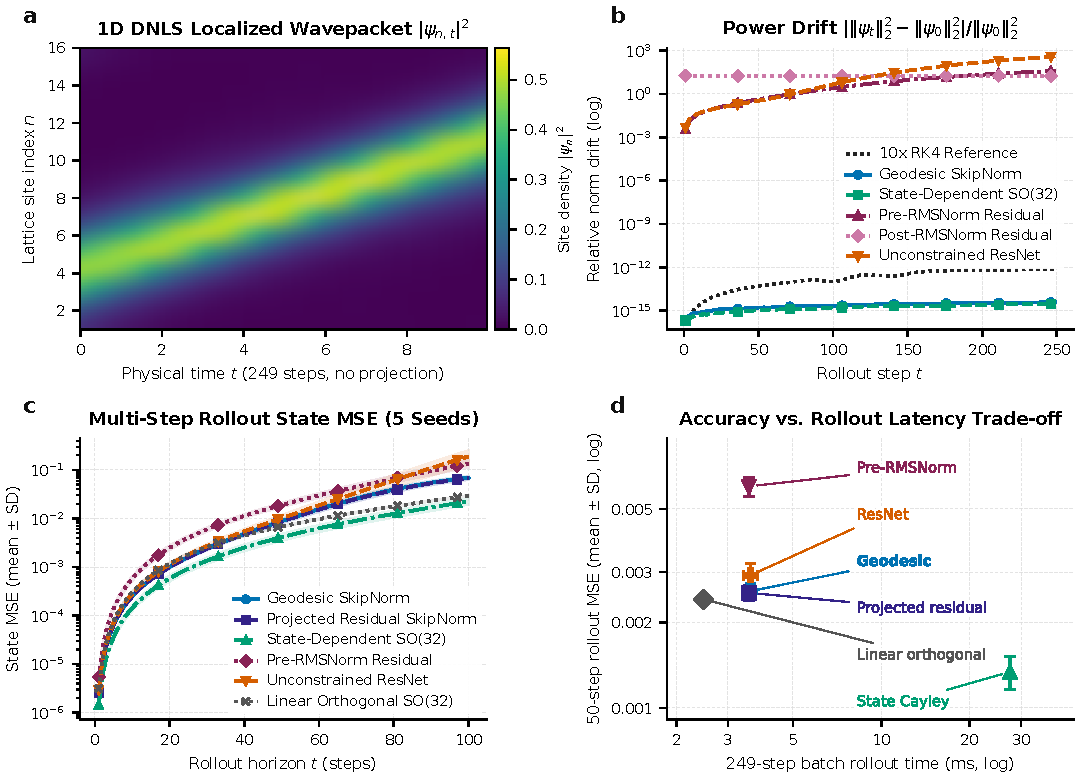
\includegraphics[width=\textwidth]{fig2_dnls_unitary_rollout.pdf}
\caption{Conservation and prediction on DNLS. (a) Reference density of the fixed held-out illustrative wave packet. (b) Relative power drift, averaged over test trajectories and training seeds; values below $10^{-16}$ are displayed at that plotting threshold. (c) Per-step state MSE, mean $\pm$ sample SD across five seeds. (d) Cumulative MSE@50 versus warm batch inference time. Timings compare the specified implementations and parameter budgets, not all possible orthogonal parameterizations.}
\label{fig:dnls}
\end{figure}

All models use the same eight-step prediction objective, training windows, and 900 optimizer updates. The nonlinear branches have two hidden layers of width 96. The state-dependent orthogonal baseline predicts two $32\times4$ factors and applies a dense Cayley solve to their skew-symmetric product; it has more parameters than the vector-field models. The fixed linear orthogonal baseline is smaller. Table~\ref{tab:dnls_results} reports these budgets explicitly; full settings and timing procedures appear in Appendix~\ref{app:protocols}.

The norm-preserving models maintain power near floating-point precision, as expected from their construction. This does not make their trajectories more accurate than the reference solver. The projected-residual and tangent-projected updates have similar prediction errors in this benchmark. The dense state-dependent Cayley model is more accurate at short and intermediate horizons but costs more per rollout; the linear orthogonal model is faster and has lower cumulative error at horizon 200 than Geodesic SkipNorm. The experiment therefore supports a computational trade-off, rather than a general accuracy advantage for the spherical retraction. The geometric exclusion of an antipodal flip in Proposition~\ref{prop:geodesic_skipnorm} is a separate property; it does not establish a performance advantage when such flips are absent from training.

\section{Conditional Radial Foliation of Conserved Quantities}
\label{sec:foliation}

In general conservative systems (such as Lotka--Volterra population dynamics or anharmonic oscillators), the conserved quantity $I(x)$ is \emph{not} the Euclidean norm $\norm{x}_2$ in observed coordinates. Consider a dynamical autoencoder $(E, g, D)$ with encoder $E: \mathcal{M} \to \R^{d_z}$, norm-preserving latent transition $g: \R^{d_z} \to \R^{d_z}$ ($\norm{g(z)}_2 = \norm{z}_2$, implemented via Geodesic SkipNorm or $\mathrm{SO}(d_z)$), and decoder $D: \R^{d_z} \to \mathcal{M}$. We give sufficient conditions under which intertwining the observed flow $\Phi_{\Delta t}$ with $g$ forces the latent radius $h(x) \coloneqq \norm{E(x)}_2$ to foliate the level sets of $I$.

\subsection{The Conditional Radial Foliation Theorem}

\begin{theorem}[Conditional Radial Foliation of Connected Regular Level Sets]
\label{thm:radial_foliation}
Let $U\subseteq\R^N$, $N\ge2$, be open, and let $I\in C^1(U,\R)$ satisfy $I\circ\Phi_{\Delta t}=I$ for a time-step map $\Phi_{\Delta t}:U\to U$. Let $J=(c_{\min},c_{\max})\subseteq I(U)$ and write $\mathcal O_c=I^{-1}(c)$. Suppose:
\begin{enumerate}
    \item[\textbf{(H1)}] $E:U\to\R^{d_z}$ is continuous, $\norm{g(z)}_2=\norm z_2$ on $E(U)$, and $E\circ\Phi_{\Delta t}=g\circ E$ on $U$.
    \item[\textbf{(H2)}] Each $c\in J$ is a regular value of $I$ and $\mathcal O_c$ is connected. There is a dense subset $J_*\subseteq J$ such that each $\mathcal O_c$, $c\in J_*$, contains a point with a dense forward orbit under the \emph{sampled map} $\Phi_{\Delta t}$.
\end{enumerate}
Then:
\begin{enumerate}
    \item[\textbf{(a)}] \textbf{Radial constancy and continuity.} For arbitrary $d_z\ge1$, there is a unique continuous $\psi:J\to\R_{\ge0}$ such that
    \begin{equation}
        \norm{E(x)}_2=\psi(I(x))\quad(x\in I^{-1}(J)),\qquad
        E(\mathcal O_c)\subseteq\Sp^{d_z-1}(\psi(c)).
        \label{eq:level_set_constancy}
    \end{equation}
    A radius-zero sphere here denotes the singleton $\{0\}$.
    \item[\textbf{(b)}] \textbf{Dimension-matched identification.} Assume additionally:
    \begin{enumerate}
        \item[\textbf{(H3)}] $d_z=N$, every $\mathcal O_c$ is compact, and $E$ is globally injective on $U$.
    \end{enumerate}
    Then $\psi(c)>0$, each $E|_{\mathcal O_c}$ is a homeomorphism onto the entire sphere $\Sp^{N-1}(\psi(c))$, and $\psi$ is a strictly monotone homeomorphism from $J$ onto an open interval in $\R_{>0}$.
\end{enumerate}
\end{theorem}

For $c\in J_*$, norm preservation and intertwining make $h=\norm{E(\cdot)}_2$ constant on a dense orbit, hence on its level set. Local sections of the submersion $I$ extend this constancy to every regular level and establish continuity of $\psi$. Under (H3), invariance of domain and compactness force each encoded level set to fill its target sphere; global injectivity then makes distinct levels have distinct radii. Appendix~\ref{app:foliation_proofs} gives the proof. The conclusion is strict monotonicity, with either orientation; an increasing orientation requires additional geometric information.

The dense-label formulation accommodates isolated or lower-dimensional sets of resonant labels. For a periodic continuous-time orbit with period $T(c)$, density of the sampled orbit requires $\Delta t/T(c)\notin\mathbb Q$. Continuous-time orbit coverage alone is insufficient. We do not assume that every level of a nonisochronous oscillator satisfies this condition.

\paragraph{A control without level-set orbit density.}
Suppose $N = 4$ and a 4D phase space has a single scalar energy $H(q_1, p_1, q_2, p_2) = \frac{1}{2}(q_1^2 + p_1^2) + \frac{1}{2}(q_2^2 + p_2^2) = H_1 + H_2$, so each energy shell $\mathcal{O}_c \cong \Sp^3(\sqrt{2c})$ is compact, connected, and regular, \emph{but} every continuous-time orbit is periodic ($1:1$ resonance), and each sampled orbit is contained in a 1D circle $\Sp^1$ that is nowhere dense in $\Sp^3(\sqrt{2c})$. Consider the analytical diffeomorphism $E(q_1, p_1, q_2, p_2) = (\sqrt{2}q_1, \sqrt{2}p_1, q_2, p_2)$ intertwined with the exact block-rotation $g \in \mathrm{SO}(4)$. As verified in Figure~\ref{fig:obstructions}c and Appendix~\ref{app:foliation_proofs}:
\begin{equation}
    E \circ \Phi_{\Delta t} = g \circ E \;\; (\text{exact}), \qquad \CV_{\mathcal{O}}(h) = 0 \;\; (\text{zero within-orbit wobble}),
\end{equation}
yet on the single energy shell $H = 1$, the encoded radius $\norm{E(x)}_2 = \sqrt{2 H_1 + 2 H} = \sqrt{2(1 + \eta)}$ varies continuously with the mode energy partition $\eta = H_1 / H \in [0, 1]$ from $\sqrt{2} \approx 1.414$ to $2.000$ (a nonzero spread across orbits on the same level set). Thus, without (H2), intertwining only forces $\norm{E(x)}_2$ to be an orbit invariant, not a function of $H$ alone.

\subsection{Evaluation Metrics and Trajectory Splits}
\label{sec:metrics}

All foliation metrics use encoded \emph{reference} trajectories $z_{m,t}=E(x_{m,t})$, not generated latent trajectories, whose norms are constrained by construction. For a scalar radius $r_{m,t}=\norm{z_{m,t}}_2$, write $\bar r_m=T^{-1}\sum_t r_{m,t}$ and $s_m^2=T^{-1}\sum_t(r_{m,t}-\bar r_m)^2$. We report the average within-trajectory coefficient of variation $M^{-1}\sum_m s_m/\max(\bar r_m,10^{-15})$, together with the within/total variance ratio
\begin{equation}
 W=\frac1M\sum_m s_m^2,\quad B=\Var_m(\bar r_m),\qquad
 \OVR=\frac{W}{W+B}.
 \label{eq:ovr_def}
\end{equation}
The training-centered latent scale is $\sigma_{\mathrm{lat}}^2=\mathbb E_{\mathrm{train}}\norm{z-\mathbb E_{\mathrm{train}}z}_2^2$. We mark OVR undefined when $\sigma_{\mathrm{lat}}=0$, or when either $B$ or $W+B$ is at most $(10^{-4}\sigma_{\mathrm{lat}})^2$. The component variances are saved with each run. CV near a zero mean is not a reliable identification measure; neither CV nor OVR alone establishes invariant recovery.

For scalar foliation, isotonic regression estimates the forward calibration $c\mapsto\bar r$: its direction and knots are fitted on training trajectories only, then linearly interpolated at test labels, with constant boundary extension outside the training range. Test $R^2$ compares these predicted radii with test mean radii. This is a calibration of the foliation function, not an inverse readout of the physical invariant from an individual state. We separately report test Spearman $|\rho_S|$. For multiple invariants we fit a degree-two ridge readout from radii to the invariant vector, using training-only standardization and a fixed penalty $10^{-4}$. Test $R^2$ is never clipped to zero. Physical invariant labels enter these post-training evaluations only.

\begin{table}[t]
\centering
\caption{Lotka--Volterra evaluation on 16 held-out trajectories. All models predict over the same physical horizon $1.8$, with five-seed mean $\pm$ sample SD. Calib.\ $R^2$ predicts mean radius from the invariant using a training-fitted isotonic map. The projected-invariant baseline learns a scalar with an arbitrary offset; its CV is omitted because that gauge is not comparable to an encoder norm. Its OVR and calibration use that learned scalar.}
\label{tab:lv_results}
\resizebox{\textwidth}{!}{% Generated by experiments/export_paper_tables.py; do not edit.
% Source SHA-256: results/stage1/stage1_results.json 81341d024c4ca00e6f7370ecdc1946dfe13894f13868559ba00dc4c0ba4dc0ab
% Source SHA-256: results/stage2/stage2_results.json cb1f24dd8d99bd50638b720c69ee00580abb85c8a6204cf854378fc7f4b08414
% Source SHA-256: results/stage3/stage3_dnls_results.json 83bc144c140c31ceef32a5f34154fb33699cff162cea1e8a9bf345c7e594c10f
% Source SHA-256: results/submission_validation.json 634aeee8c56dc63057afea9d4815d77a8b35853bf3e8c84efb23265e33964531
% Source SHA-256: data/splits/splits_manifest.json 8036304e05a83fc8aaa3db088b368461db7b6d05ba3009d7d558740d177e39c8
% Exporter SHA-256: 79d377a480ab670d4ae41b1072098e14c3d75bdd73e5e2301487606a64150516
% Calibration predicts mean radius from the invariant, fitted on training trajectories.
% Projected-invariant CV is omitted: its scalar offset makes it incomparable to encoder radius CV.
% Rollout: 12 coarse steps, stride=3, physical horizon=1.8; legacy JSON field ends in _20.
\begin{tabular}{lrrrrr}
\toprule
Model & CV & OVR & Calib. $R^2$ & $|\rho|$ & Rollout MSE \\
\midrule
GSN: bijective, radial & $0.0135 \pm 0.0052$ & $(1.89 \pm 1.3)\times 10^{-3}$ & $0.999950 \pm 1.2\times 10^{-6}$ & $1.000000 \pm 0$ & $(1.01 \pm 0.47)\times 10^{-3}$ \\
GSN: MLP, radial & $0.0265 \pm 0.0031$ & $(4.86 \pm 1.4)\times 10^{-3}$ & $0.999970 \pm 4.1\times 10^{-6}$ & $1.000000 \pm 0$ & $(2.78 \pm 0.96)\times 10^{-3}$ \\
Projected residual & $0.0148 \pm 8.4\times 10^{-4}$ & $(1.69 \pm 0.21)\times 10^{-3}$ & $0.999962 \pm 2.3\times 10^{-6}$ & $1.000000 \pm 0$ & $(2.52 \pm 0.64)\times 10^{-4}$ \\
State-dependent $\mathrm{SO}(2)$ & $0.0141 \pm 0.0012$ & $(1.46 \pm 0.19)\times 10^{-3}$ & $0.999960 \pm 5.2\times 10^{-6}$ & $1.000000 \pm 0$ & $(1.94 \pm 0.47)\times 10^{-4}$ \\
Projected invariant & -- & $0.633 \pm 0.36$ & $0.999843 \pm 1.6\times 10^{-4}$ & $1.000000 \pm 0$ & $0.291 \pm 0.3$ \\
Unconstrained AE & $0.154 \pm 0.0068$ & $0.22 \pm 0.012$ & $0.999973 \pm 1.7\times 10^{-6}$ & $1.000000 \pm 0$ & $(2.16 \pm 0.44)\times 10^{-4}$ \\
\bottomrule
\end{tabular}
}
\end{table}

\begin{figure}[t]
\centering
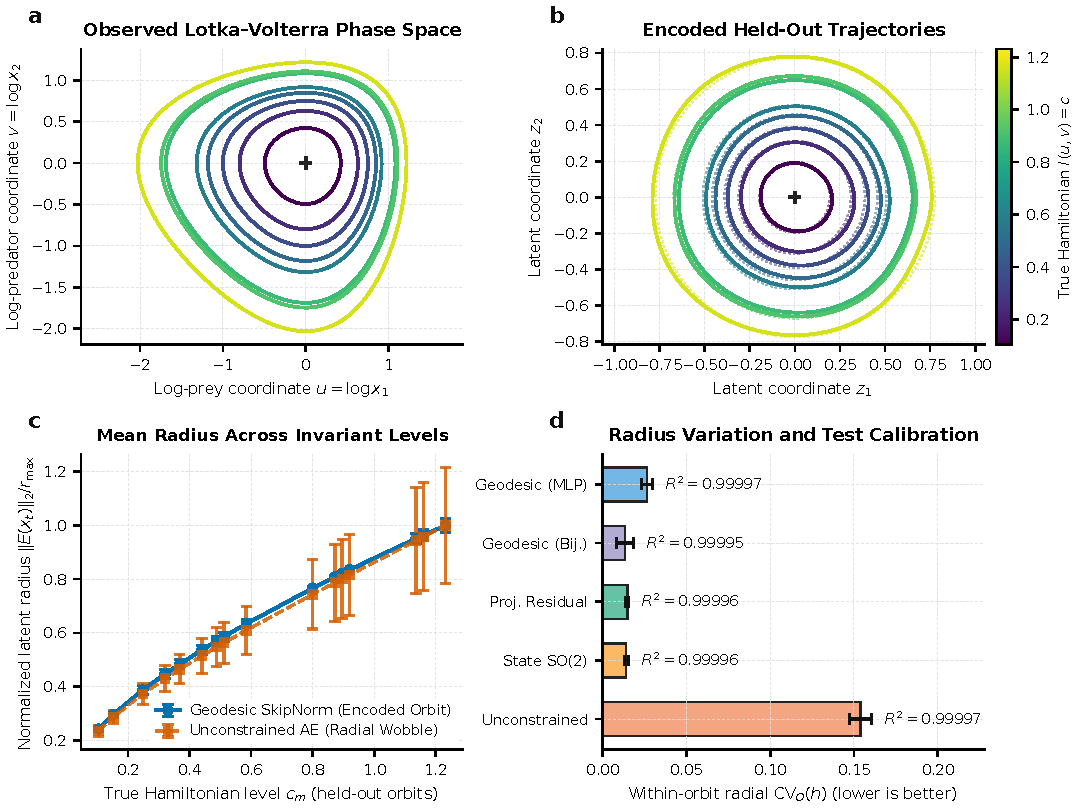
\includegraphics[width=\textwidth]{fig3_scalar_foliation_lotka_volterra.pdf}
\caption{Scalar foliation on Lotka--Volterra test trajectories. (a) Reference trajectories in log-population coordinates, colored by the conserved Hamiltonian. (b) Seed-zero MLP encodings; dotted circles are mean-radius guides. Observed and encoded curves are sampled trajectories, trimmed to at most one revolution without adding closing segments. (c) Test mean radius versus invariant, scaled by each model's maximum test mean radius for display; error bars show within-trajectory SD. (d) Encoder radial CV across training seeds and training-fitted test radius-calibration $R^2$. These finite-data observations illustrate approximate foliation and do not certify the exact theorem's hypotheses.}
\label{fig:lv_foliation}
\end{figure}

\paragraph{Lotka--Volterra experiment.}
In log-population coordinates, $\dot u=1-e^v$, $\dot v=e^u-1$ preserves $I(u,v)=e^u-u+e^v-v-2$. Its positive level sets are compact, connected curves surrounding $(0,0)$. We use 32 training, 8 validation, and 16 test trajectories of 180 states at $\Delta t=0.05$. The norm-preserving autoencoders in Table~\ref{tab:lv_results} reduce radial variation relative to the unconstrained autoencoder, although a monotone mean-radius calibration can also be learned without imposing norm preservation. Reconstruction, prediction, radial constancy, and cross-level ordering are therefore distinct outcomes.

The two-dimensional Geodesic models use a radius-dependent frequency network multiplying $(-z_2,z_1)$; this imposes phase-independent angular dynamics in addition to norm preservation. The other MLP transitions use general state-dependent vector fields, while the state-dependent orthogonal model predicts a Cayley matrix. We also include a trajectory-trained projected-invariant baseline inspired by COMET's gradient projection \citep{otto2023learning}. Its supervision, integrator, and regularization differ from the original method, so these results are not a reproduction of COMET. Architecture and loss details are given in Appendix~\ref{app:protocols}.

\section{Topological Obstructions on Multi-Basin Phase Spaces}
\label{sec:obstructions}

What happens when the connectedness hypothesis (H2) of Theorem~\ref{thm:radial_foliation} is violated, as in a double-well Hamiltonian $H(q, p) = \frac{1}{2}p^2 - \frac{1}{2}q^2 + \frac{1}{4}q^4 + \gamma q$ at regular energies above both well minima and below the saddle energy, where each level set $\mathcal{O}_c = \mathcal{O}_c^{(1)} \sqcup \mathcal{O}_c^{(2)}$ is the disjoint union of a left-well loop ($q < q_{\mathrm{saddle}}$) and a right-well loop ($q > q_{\mathrm{saddle}}$)?

\begin{theorem}[Jordan--Brouwer Obstruction for Disjoint Enclosed Basins]
\label{thm:jordan_brouwer}
Let $U\subseteq\R^N$, $N\ge2$, be open. Let $\Sigma_1,\Sigma_2\subset U$ be disjoint embedded copies of $\Sp^{N-1}$ with disjoint bounded complementary domains $B_1,B_2$ and $\overline B_1\cup\overline B_2\subset U$. If $E:U\to\R^N$ is continuous and injective, then
\begin{enumerate}
    \item[\textbf{(a)}] $E(B_i)$ is the bounded complementary domain of $E(\Sigma_i)$ for $i=1,2$, and these two domains are disjoint. In particular, both encoded boundaries cannot enclose the origin.
    \item[\textbf{(b)}] $E(\Sigma_1)$ and $E(\Sigma_2)$ cannot both be origin-centered spheres, even with distinct radii. Equivalently, $\norm{E(\cdot)}_2$ cannot be constant on both boundaries.
\end{enumerate}
\end{theorem}

For scalar periodic level curves in the plane, the theorem applies when both enclosed wells are included in the encoder domain. If exact intertwining and sampled-orbit density would force both boundaries to have constant encoded radius, they are incompatible with such a globally injective encoder. This is an exact obstruction, with no quantitative lower bound on finite-sample CV or prediction error.

\paragraph{Encoder regimes and a translation control.}
An unconstrained encoder can lose injectivity, whereas a bijective encoder can produce nonconstant radii or place the images away from the origin. These are possible behaviors, not an exhaustive classification or a theorem about training outcomes. Low CV alone cannot distinguish them. In particular, for trajectories in a compact set with $\norm x_2\le R$ and $\norm{\Phi_{\Delta t}(x)-x}_2\le D$, the injective translated encoder $E_a(x)=ae_1+x$, $a>R$, and identity transition $g(z)=z$ satisfy
\begin{equation}
    \CV_{\mathcal O}(\norm{E_a}_2)\le\frac{R}{a-R},\qquad
    \frac{\norm{E_a(\Phi_{\Delta t}(x))-g(E_a(x))}_2}{\norm{E_a(x)}_2}\le\frac{D}{a-R}.
    \label{eq:translated_control}
\end{equation}
Here CV uses the standard deviation under an empirical or population probability measure on the trajectory. Both quantities can approach zero while the absolute prediction displacement remains unchanged. The images lie near a sphere of large radius, not exactly on it; the bound does not contradict Theorem~\ref{thm:jordan_brouwer}.



\begin{table}[t]
\centering
\caption{Double-well controls, five-seed mean $\pm$ sample SD. ``Both'' is the percentage of seeds with at least one left and one right test polygon enclosing the origin, evaluated across all 16 test curves; it is not a certificate of global injectivity. Global and within-well $R^2$ are training-fitted radius calibrations, with the latter averaged equally across wells; well-probe accuracy uses a radius threshold and orientation selected on training data. The reflection-quotient control uses a different reconstruction task and is evaluated only for symmetric potentials.}
\label{tab:double_well_results}
\resizebox{\textwidth}{!}{% Generated by experiments/export_paper_tables.py; do not edit.
% Source SHA-256: results/stage1/stage1_results.json 81341d024c4ca00e6f7370ecdc1946dfe13894f13868559ba00dc4c0ba4dc0ab
% Source SHA-256: results/stage2/stage2_results.json cb1f24dd8d99bd50638b720c69ee00580abb85c8a6204cf854378fc7f4b08414
% Source SHA-256: results/stage3/stage3_dnls_results.json 83bc144c140c31ceef32a5f34154fb33699cff162cea1e8a9bf345c7e594c10f
% Source SHA-256: results/submission_validation.json 634aeee8c56dc63057afea9d4815d77a8b35853bf3e8c84efb23265e33964531
% Source SHA-256: data/splits/splits_manifest.json 8036304e05a83fc8aaa3db088b368461db7b6d05ba3009d7d558740d177e39c8
% Exporter SHA-256: 79d377a480ab670d4ae41b1072098e14c3d75bdd73e5e2301487606a64150516
% Calibration predicts mean radius from energy; each fit uses training trajectories only.
% Both is the across-seed rate of both well families having a sampled polygon enclosing zero.
% Well probe is held-out accuracy of a training-fitted radius threshold/orientation.
% Reflection quotient is deliberately absent for the tilted potential.
\begin{tabular}{lrrrrrr}
\toprule
Encoder & CV & OVR & Global $R^2$ & Within $R^2$ & Both (\%) & Probe (\%) \\
\midrule
\multicolumn{7}{l}{\emph{Symmetric, balanced training}} \\
Origin-pinned bijective & $0.281 \pm 0.023$ & $0.782 \pm 0.032$ & $0.812364 \pm 0.2$ & $0.998902 \pm 3.9\times 10^{-4}$ & $0 \pm 0$ & $60 \pm 3.4$ \\
Reflection quotient & $0.0812 \pm 0.0025$ & $0.087 \pm 0.0076$ & $0.999980 \pm 9.3\times 10^{-7}$ & $0.999782 \pm 2.1\times 10^{-5}$ & $100 \pm 0$ & $50 \pm 0$ \\
Free-shift bijective & $0.118 \pm 0.09$ & $0.485 \pm 0.33$ & $0.334756 \pm 0.49$ & $0.998101 \pm 7.5\times 10^{-4}$ & $0 \pm 0$ & $81.2 \pm 21$ \\
\midrule
\multicolumn{7}{l}{\emph{Symmetric, imbalanced training}} \\
Origin-pinned bijective & $0.272 \pm 0.019$ & $0.647 \pm 0.11$ & $0.643684 \pm 0.15$ & $0.823188 \pm 0.033$ & $0 \pm 0$ & $56.2 \pm 14$ \\
Reflection quotient & $0.105 \pm 0.0054$ & $0.0914 \pm 0.01$ & $0.999988 \pm 9.7\times 10^{-7}$ & $0.520958 \pm 0.015$ & $100 \pm 0$ & $50 \pm 0$ \\
Free-shift bijective & $0.163 \pm 0.06$ & $0.418 \pm 0.36$ & $-0.372183 \pm 1$ & $0.681742 \pm 0.12$ & $0 \pm 0$ & $78.8 \pm 26$ \\
\midrule
\multicolumn{7}{l}{\emph{Tilted, $\gamma=0.08$}} \\
Origin-pinned bijective & $0.226 \pm 0.029$ & $0.705 \pm 0.092$ & $0.402459 \pm 0.33$ & $0.995867 \pm 0.0036$ & $0 \pm 0$ & $36.2 \pm 6.8$ \\
Free-shift bijective & $0.0615 \pm 0.025$ & $0.461 \pm 0.22$ & $0.232323 \pm 0.24$ & $0.995362 \pm 0.0031$ & $0 \pm 0$ & $100 \pm 0$ \\
\bottomrule
\end{tabular}
}
\end{table}

\begin{figure}[t]
\centering
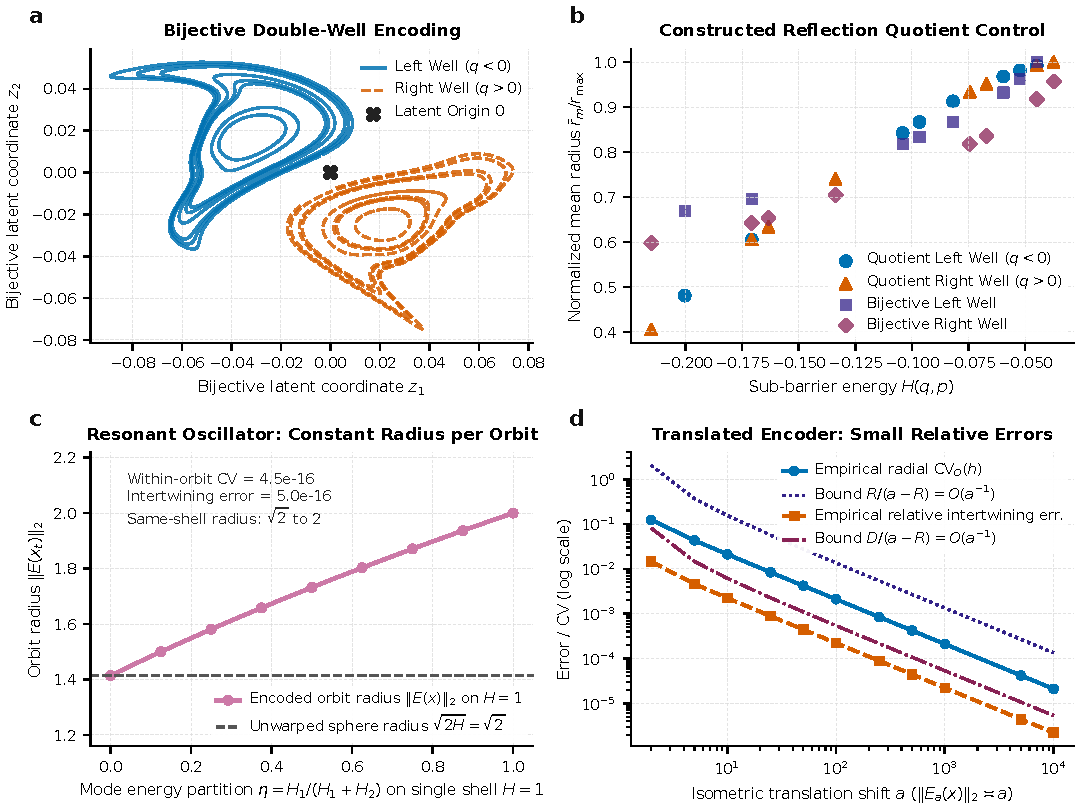
\includegraphics[width=\textwidth]{fig4_topological_obstructions_and_controls.pdf}
\caption{Obstructions and controls. (a) Encoded test segments from a bijective double-well model. (b) Mean radii from the bijective encoder and an explicitly reflection-invariant quotient encoder on the symmetric potential. The latter's noninjectivity is imposed, rather than inferred from radius overlap. (c) The exact linear resonance control has constant radius along each orbit but radii ranging from $\sqrt2$ to $2$ on the same energy shell. (d) For the translated identity encoder, small CV and relative intertwining error arise without informative decoded dynamics.}
\label{fig:obstructions}
\end{figure}

The double-well experiments use $H(q,p)=p^2/2-q^2/2+q^4/4+\gamma q$. We compare a bijective coupling encoder centered at the origin with a free-offset bijective encoder under balanced and imbalanced sampling for $\gamma=0$, and under a tilted potential $\gamma=0.08$. In the symmetric cases we additionally construct an even encoder
\begin{equation}
 E_{\mathrm{quot}}(x)=\tfrac12\bigl(A_\theta(x)+A_\theta(-x)\bigr)-A_\theta(0),
 \qquad E_{\mathrm{quot}}(x)=E_{\mathrm{quot}}(-x),
\end{equation}
and reconstruct only up to the equivalence $x\sim-x$. This control demonstrates how discarding the basin label changes the representation problem; it does not establish spontaneous folding under an ordinary reconstruction objective. Reflection is not a symmetry of the tilted Hamiltonian, so the quotient control is omitted there. A radius-only well probe measures separability in that scalar statistic, not in the full latent vector. Table~\ref{tab:double_well_results} reports finite-trajectory diagnostics; the theorem itself supplies no numerical CV floor. In the tilted case, the free-shift encoder has radial CV $0.0615\pm0.025$, yet its global calibration is only $R^2=0.232\pm0.24$. Within-well calibration remains high, illustrating how separately ordered basin coordinates need not define a single well-calibrated radius function of energy. The imbalanced free-shift model has negative mean global calibration $R^2$; these failures are retained.

\section{Toroidal Generalization: $K$-Block SkipNorm on $\bigoplus_{k=1}^K \R^{d_k}$}
\label{sec:torus}

A compact connected regular common level set of $K$ independent commuting integrals in a $2K$-dimensional Hamiltonian system is a torus under the Liouville--Arnold hypotheses \citep{arnold1989mathematical}. The results below assume the torus fibers directly and do not require Hamiltonian dynamics or canonical observations. Preserving one total norm supplies one scalar invariant; it does not prevent invariant tori from being embedded inside a sphere. For multiple architectural invariants, partition the latent state into $K$ blocks:
\begin{equation}
    g_{\mathrm{block}}(z)\coloneqq
    \left(\operatorname{GeodSkipNorm}_{\alpha_k}(z^{(k)};f^{(k)}(z))\right)_{k=1}^K.
    \label{eq:kblock_skipnorm}
\end{equation}
Each branch may depend on the full state. On nonzero blocks the update preserves every $\rho_k(z)=\norm{z^{(k)}}_2$; zero blocks may be assigned zero output. Blocks of dimensions $d_k$ preserve a product of spheres $\prod_k\Sp^{d_k-1}(\rho_k)$. The toroidal identification theorem specifically uses $d_k=2$ for every block.

\begin{theorem}[Scalar Non-Identifiability and Planar-Block Toroidal Foliation]
\label{thm:toroidal_kblock}
Let $U\subseteq\R^{2K}$ and $\Omega\subseteq\R^K$ be nonempty open sets, with $K\ge2$. Let $\Phi_{\Delta t}:U\to U$, and let $I:U\to\Omega$ be a surjective $C^1$ submersion satisfying $I\circ\Phi_{\Delta t}=I$. Suppose each fiber $\mathcal O_c=I^{-1}(c)$ is a compact connected $K$-torus, and for a dense subset $\Omega_*\subseteq\Omega$ each fiber has a dense forward orbit under $\Phi_{\Delta t}$. Let $E$ be continuous and satisfy exact intertwining with the specified latent transition.
\begin{enumerate}
    \item[\textbf{(a)}] \textbf{One scalar radius cannot identify all invariant labels.} If $g$ preserves the total norm, then $\norm{E(x)}_2=\psi(I(x))$ for a continuous $\psi:\Omega\to\R_{\ge0}$. This map cannot be injective, so no readout from the total radius can recover every label in $\Omega$ exactly. This conclusion places no universal upper bound on statistical readout $R^2$.
    \item[\textbf{(b)}] \textbf{Identification by $K$ planar block radii.} Suppose $E:U\to\bigoplus_{k=1}^K\R^2$ is globally injective and $g$ preserves each block norm. Then there is a continuous map $\Psi:\Omega\to\R_{>0}^K$ such that
    \begin{equation}
        \bm\rho(E(x))=\Psi(I(x)),\qquad
        E(\mathcal O_c)=\prod_{k=1}^K\Sp^1(\psi_k(c)).
        \label{eq:toroidal_foliation}
    \end{equation}
    Each restricted encoder is a homeomorphism onto this product of circles, and $\Psi$ is a homeomorphism onto its open image in $\R_{>0}^K$. Thus the vector of block radii identifies the invariant labels up to a continuous change of coordinates.
\end{enumerate}
\end{theorem}

The proof in Appendix~\ref{app:obstruction_proofs} first extends radial constancy from the dense set of labels using local sections. Global injectivity excludes zero block radii, and invariance of domain gives surjectivity on each product of circles and invertibility of $\Psi$. No differentiability of $E$ or $\Psi$ is needed. These coordinates need not equal canonical actions, and the result does not guarantee that a chosen finite-capacity readout can invert them. The scalar limitation concerns recovery from the total radius alone: even a single-sphere model can represent a torus, for example through the Clifford embedding $(\theta_1,\ldots,\theta_K)\mapsto K^{-1/2}(\cos\theta_1,\sin\theta_1,\ldots,\cos\theta_K,\sin\theta_K)$ into $\Sp^{2K-1}$.


\begin{table}[t]
\centering
\caption{Two-invariant oscillator experiment: 20 held-out trajectories, five-seed mean $\pm$ sample SD. Total and block CV use encoded reference trajectories. Scalar and two-block $R^2$ use training-fitted degree-two ridge readouts of $(I_1,I_2)$; negative scores are retained. The radius-frequency (RF) and general-vector-field (VF) two-block models distinguish the architectural frequency prior from blockwise norm preservation. Rollout MSE covers the same physical horizon $2.88$ for all models.}
\label{tab:torus_results}
\resizebox{\textwidth}{!}{% Generated by experiments/export_paper_tables.py; do not edit.
% Source SHA-256: results/stage1/stage1_results.json 81341d024c4ca00e6f7370ecdc1946dfe13894f13868559ba00dc4c0ba4dc0ab
% Source SHA-256: results/stage2/stage2_results.json cb1f24dd8d99bd50638b720c69ee00580abb85c8a6204cf854378fc7f4b08414
% Source SHA-256: results/stage3/stage3_dnls_results.json 83bc144c140c31ceef32a5f34154fb33699cff162cea1e8a9bf345c7e594c10f
% Source SHA-256: results/submission_validation.json 634aeee8c56dc63057afea9d4815d77a8b35853bf3e8c84efb23265e33964531
% Source SHA-256: data/splits/splits_manifest.json 8036304e05a83fc8aaa3db088b368461db7b6d05ba3009d7d558740d177e39c8
% Exporter SHA-256: 79d377a480ab670d4ae41b1072098e14c3d75bdd73e5e2301487606a64150516
% Readouts predict the two invariants from one total radius or two planar block radii.
% Degree-two ridge uses training standardization/fit; negative held-out R2 is retained.
% Rollout: 12 coarse steps, stride=3, physical horizon=2.88; legacy JSON field ends in _20.
\begin{tabular}{lrrrrrr}
\toprule
Model & Total CV & Block CV & Block OVR & $R^2_1$ & $R^2_2$ & Rollout MSE \\
\midrule
Two blocks (RF) & $0.0114 \pm 8.4\times 10^{-4}$ & $0.0187 \pm 0.0013$ & $(8.29 \pm 1.6)\times 10^{-3}$ & $0.137308 \pm 0.021$ & $0.999322 \pm 1.1\times 10^{-4}$ & $(3.77 \pm 0.78)\times 10^{-3}$ \\
Two blocks (VF) & $0.167 \pm 0.071$ & $0.27 \pm 0.12$ & $0.529 \pm 0.23$ & $-0.001223 \pm 0.1$ & $0.304673 \pm 0.36$ & $0.23 \pm 0.14$ \\
Single sphere & $0.036 \pm 0.0017$ & $0.321 \pm 0.055$ & $0.734 \pm 0.17$ & $0.174985 \pm 0.019$ & $0.519861 \pm 0.33$ & $0.0467 \pm 0.002$ \\
Unconstrained AE & $0.093 \pm 0.0095$ & $0.353 \pm 0.039$ & $0.817 \pm 0.06$ & $0.158983 \pm 0.0098$ & $0.326286 \pm 0.24$ & $0.0495 \pm 0.0024$ \\
\bottomrule
\end{tabular}
}
\end{table}

\begin{figure}[t]
\centering
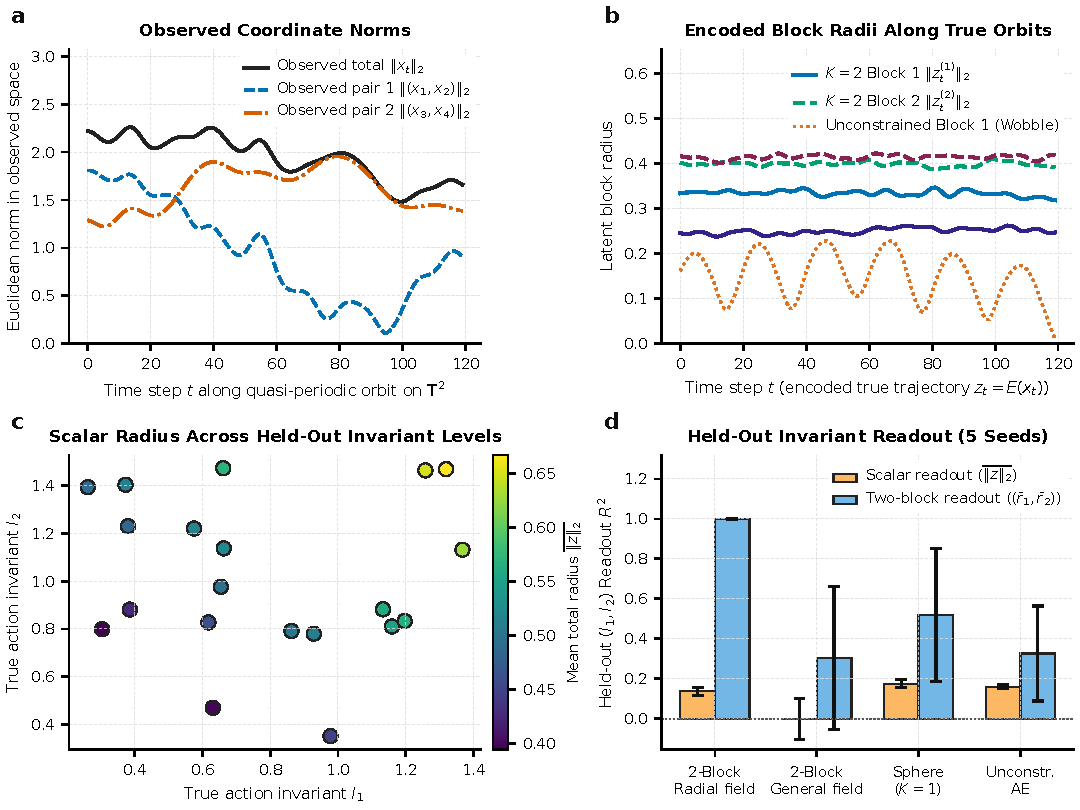
\includegraphics[width=\textwidth]{fig5_toroidal_kblock_foliation.pdf}
\caption{Toroidal representation experiment. (a) Observed coordinate norms along a test trajectory. (b) Encoded planar block radii along reference trajectories for the radius-frequency two-block model and unconstrained baseline. (c) True test invariant labels colored by the time-mean total latent radius. (d) Test readout $R^2$ from one total radius or two block radii, with sample SD across five seeds, including the general-vector-field ablation. There is no universal statistical $R^2$ ceiling for a scalar readout; the theorem concerns exact identification over an open invariant domain.}
\label{fig:torus}
\end{figure}

\paragraph{Coupled oscillator experiment.}
Two hidden invariants $(I_1,I_2)\in[0.25,1.5]^2$ determine the frequencies
\begin{equation}
 \omega_1=1+0.5I_1+0.25I_2,\qquad
 \omega_2=\sqrt2+0.25I_1+0.40I_2.
\end{equation}
They are the derivatives of $\mathcal H(I)=I_1+\sqrt2 I_2+0.25I_1^2+0.20I_2^2+0.25I_1I_2$. A fixed smooth invertible observation map mixes the oscillator coordinates; it is not asserted to be canonical. There are 44 training, 8 validation, and 20 test trajectories, each containing 120 states at $\Delta t=0.08$. The frequency map has nonsingular Jacobian. Nonresonant sampled frequencies form a dense set of invariant labels, consistent with the density hypothesis in Theorem~\ref{thm:toroidal_kblock}; finite observed segments do not themselves certify dense coverage.

The radius-frequency two-block model predicts each angular rate from both block radii. Its phase-independent frequency prior is stronger than blockwise norm conservation alone. The general-vector-field ablation instead applies two-block retraction to an unrestricted four-dimensional MLP output, using the same encoder, decoder, width, training objective, and number of updates. The one-sphere and unconstrained baselines also use general vector fields. The radius-frequency model attains two-block readout $R^2=0.9993\pm0.0001$, whereas the general-vector-field variant attains $0.305\pm0.358$ and has substantially larger reference-encoding block CV ($0.270\pm0.116$ versus $0.0187\pm0.0013$). Its rollout error is also larger. Thus blockwise preservation alone did not reproduce the strongest recovery under the same training schedule; the result supports the combined radius-frequency architecture. This ablation does not establish that a general vector field cannot learn a comparable representation with another training procedure. The difference is an empirical optimization result, not a numerical consequence of the topological theorem.

\section{Discussion, Limitations, and Conclusion}
\label{sec:discussion}

The identification results require exact intertwining, regular fibers with sampled-orbit density on a dense set of labels, and global injectivity when distinct invariant levels must be separated. Finite-horizon prediction and low radius CV do not establish these hypotheses. Resonances can invalidate orbit density on a fiber; chaotic dynamics may satisfy density on some invariant sets, so chaos alone is not an exclusion criterion. The compact regular-fiber theorems do not address singular levels, separatrices, dissipative attractors, or changing invariant dimension.

The multi-basin obstruction concerns a globally injective encoder defined on both enclosed basins. Local charts, a discrete basin label, or a different latent geometry can avoid this obstruction. The planar-block construction requires a specified number of blocks and does not by itself identify the number of physical invariants. Its homeomorphic recovery guarantee also does not select canonical actions or imply a particular finite-sample readout score. Conservation accuracy and trajectory accuracy remain separate evaluation criteria.

The empirical scope is limited to synthetic systems and five optimization seeds on one fixed split. The strongest torus readout requires the additional radius-frequency prior in the tested protocol, and low double-well radius CV can coexist with poor held-out energy-to-radius calibration. The differential identities apply exactly only away from numerical cutoffs. We therefore interpret these experiments as checks and limitations of a representation principle, rather than a general claim of superior forecasting or automatic invariant discovery.

For dissipative dynamics one could introduce a positive radial gate $\gamma(x)$ multiplying a norm-preserving map $F$. This changes the differential identity: with $r=\norm x_2$ and $u_{\mathrm{out}}=F(x)/r$, the product rule gives
\begin{equation}
    D(\gamma F)(x)^\top u_{\mathrm{out}}
    =\gamma(x)u_{\mathrm{in}}+r\nabla\gamma(x).
\end{equation}
Thus a learned state-dependent gate does not retain the original exact radial pullback. Its treatment and identification theory lie outside the present scope.

\subsubsection*{Broader Impact Statement}
This work investigates fundamental mathematical and architectural properties of normalization layers and dynamical autoencoders. It carries no direct societal or ethical risks beyond those common to foundational machine learning and scientific computing methods.

\subsubsection*{Reproducibility Statement}
Proofs are provided in Appendices~\ref{app:geometry_proofs}--\ref{app:obstruction_proofs}. The accompanying anonymized source contains JAX float64 implementations, metric regression tests, fixed dataset generators and SHA-256 split manifests, five-seed training configurations, checkpoints, predictions, and figure/table export scripts. Historical drafts and exploratory runs are excluded from the accompanying review archive; numerical revision provenance is retained. Reference-solver refinement and source-to-table checks are reproducible from the documented commands.

\bibliography{references}
\bibliographystyle{tmlr}

\newpage
\appendix

\section{Proofs of Differential Geometry Propositions and Counterexamples}
\label{app:geometry_proofs}

\subsection{Proof of Proposition~\ref{prop:skipnorm_jacobian} (Exact Jacobian Geometry of Euclidean SkipNorm)}

\begin{proof}
Let $x \in \R^{d_{\mathrm{in}}} \setminus \{0\}$ with $r = \norm{x}_2 > 0$ and $u_{\mathrm{in}} = x / r$. Since $f: \R^{d_{\mathrm{in}}} \to \R^{d_{\mathrm{out}}}$ is $C^1$ near $x$ and $y = f(x) \neq 0$, the map $u_{\mathrm{out}}(x) = f(x) / \norm{f(x)}_2$ is $C^1$ near $x$ with derivative
\begin{equation}
    D_x u_{\mathrm{out}}(x) = \frac{1}{\norm{f(x)}_2} \left( I_{d_{\mathrm{out}}} - u_{\mathrm{out}}(x) u_{\mathrm{out}}(x)^\top \right) D_x f(x).
    \label{eq:du_out_formula}
\end{equation}
Notice that $u_{\mathrm{out}}(x)^\top D_x u_{\mathrm{out}}(x) = 0$, so $\operatorname{im}(D_x u_{\mathrm{out}}(x)) \subseteq u_{\mathrm{out}}(x)^\perp$. By the product rule applied to $F(x) = r(x) u_{\mathrm{out}}(x)$ with $D_x r(x) = u_{\mathrm{in}}^\top$,
\begin{equation}
    J(x) = D_x F(x) = u_{\mathrm{out}}(x) D_x r(x) + r(x) D_x u_{\mathrm{out}}(x) = u_{\mathrm{out}} u_{\mathrm{in}}^\top + r D_x u_{\mathrm{out}}(x).
\end{equation}
Inserting the orthogonal decomposition $I_{d_{\mathrm{in}}} = u_{\mathrm{in}} u_{\mathrm{in}}^\top + P_{u_{\mathrm{in}}^\perp}$ after $r D_x u_{\mathrm{out}}(x)$ yields
\begin{equation}
    J(x) = u_{\mathrm{out}} u_{\mathrm{in}}^\top + \underbrace{r (D_x u_{\mathrm{out}}(x)) u_{\mathrm{in}}}_{B(x) \in u_{\mathrm{out}}^\perp} u_{\mathrm{in}}^\top + \underbrace{\big(r D_x u_{\mathrm{out}}(x)\big|_{u_{\mathrm{in}}^\perp}\big)}_{A_\perp(x): u_{\mathrm{in}}^\perp \to u_{\mathrm{out}}^\perp} P_{u_{\mathrm{in}}^\perp},
\end{equation}
which establishes Eq.~\eqref{eq:jacobian_block} in part~(a).

For part~(b), left-multiplying $J(x)^\top = u_{\mathrm{in}} u_{\mathrm{out}}^\top + u_{\mathrm{in}} B(x)^\top + P_{u_{\mathrm{in}}^\perp} A_\perp(x)^\top$ onto $u_{\mathrm{out}}$ and using $B(x) \in u_{\mathrm{out}}^\perp \implies B(x)^\top u_{\mathrm{out}} = 0$ and $\operatorname{im}(A_\perp(x)) \subseteq u_{\mathrm{out}}^\perp \implies A_\perp(x)^\top u_{\mathrm{out}} = 0$ gives
\begin{equation}
    J(x)^\top u_{\mathrm{out}} = u_{\mathrm{in}} (u_{\mathrm{out}}^\top u_{\mathrm{out}}) + 0 + 0 = u_{\mathrm{in}}.
\end{equation}
Hence $\norm{J(x)^\top u_{\mathrm{out}}}_2 = \norm{u_{\mathrm{in}}}_2 = 1$, and $\sigma_{\max}(J(x)) = \norm{J(x)^\top}_{\mathrm{op}} \ge \norm{J(x)^\top u_{\mathrm{out}}}_2 / \norm{u_{\mathrm{out}}}_2 = 1$. By induction over $L$ layers with radial unit vectors $u_\ell = x_\ell / \norm{x_\ell}_2$, $J_{\mathrm{total}}^\top u_L = J_1^\top \cdots J_L^\top u_L = J_1^\top \cdots J_{L-1}^\top u_{L-1} = \cdots = u_0$.

For part~(c), right-multiplying $J(x)$ onto $u_{\mathrm{in}}$ and using $P_{u_{\mathrm{in}}^\perp} u_{\mathrm{in}} = 0$ gives $J(x) u_{\mathrm{in}} = u_{\mathrm{out}} + B(x)$. Since $u_{\mathrm{out}} \perp B(x)$, $\norm{J(x) u_{\mathrm{in}}}_2^2 = 1 + \norm{B(x)}_2^2$, so $J(x) u_{\mathrm{in}} = u_{\mathrm{out}} \iff B(x) = 0$. If $f(\lambda x) = \lambda^\gamma f(x)$ for $\lambda > 0$, then $u_{\mathrm{out}}(\lambda x) = u_{\mathrm{out}}(x)$, so differentiating with respect to $\lambda$ at $\lambda = 1$ gives $B(x) = r (D_x u_{\mathrm{out}}(x)) u_{\mathrm{in}} = (D_x u_{\mathrm{out}}(x)) x = 0$. When $B(x) = 0$, $[J(x)] = \diag(1, \tilde{A})$, so $J(x)^\top J(x)$ has block-diagonal form $\diag(1, \tilde{A}^\top \tilde{A})$ with singular values $\{1\} \cup \sigma(\tilde{A})$.

For part~(d)(i), let $f(x) = R_{\log \norm{x}_2} x$ on $\R^2 \setminus \{0\}$. In polar coordinates $(r, \theta)$, $F(r, \theta) = (r \cos(\theta + \log r), r \sin(\theta + \log r))^\top$. At $x = e_1$ ($r = 1, \theta = 0$), $\partial F / \partial r = (\cos 0 - \sin 0, \sin 0 + \cos 0)^\top = (1, 1)^\top$ and $\partial F / \partial \theta = (-\sin 0, \cos 0)^\top = (0, 1)^\top$, so $J(e_1) = \begin{psmallmatrix} 1 & 0 \\ 1 & 1 \end{psmallmatrix}$. The eigenvalues of $J(e_1)^\top J(e_1) = \begin{psmallmatrix} 2 & 1 \\ 1 & 1 \end{psmallmatrix}$ satisfy $\lambda^2 - 3\lambda + 1 = 0 \implies \lambda = \frac{3 \pm \sqrt{5}}{2} = \varphi^2, \varphi^{-2}$, so $\sigma(J(e_1)) = \{\varphi, \varphi^{-1}\}$. For part~(d)(ii), $F(t) = t(\cos \log t, \sin \log t)^\top$ has $F'(1) = (1, 1)^\top$, whose singular value is $\norm{F'(1)}_2 = \sqrt{2}$, while $F'(1)^\top u_{\mathrm{out}}(1) = (1, 1)(1, 0)^\top = 1 = u_{\mathrm{in}}$.
\end{proof}

\subsection{Proof of Proposition~\ref{prop:stabilized_spectra} (Exact Rank and Stabilized Normalizer Spectra)}

\begin{proof}
\textbf{Part (a):} By Proposition~\ref{prop:skipnorm_jacobian}(a), $[J_{\mathrm{SkipNorm}}(x)] = \begin{psmallmatrix} 1 & 0 \\ b & \tilde{A} \end{psmallmatrix}$. Subtracting $b$ times the first row from the remaining rows via the invertible row operation $\begin{psmallmatrix} 1 & 0 \\ -b & I_{d_{\mathrm{out}}-1} \end{psmallmatrix} \begin{psmallmatrix} 1 & 0 \\ b & \tilde{A} \end{psmallmatrix} = \begin{psmallmatrix} 1 & 0 \\ 0 & \tilde{A} \end{psmallmatrix}$ proves $\rank(J_{\mathrm{SkipNorm}}(x)) = 1 + \rank(\tilde{A}) = 1 + \rank(A|_T)$. For unstabilized RMSNorm ($\varepsilon = 0$), $D_x (\sqrt{d} f(x)/\norm{f(x)}_2) = \frac{\sqrt{d}}{\norm{y}_2} P_\perp A$, whose rank is $\rank(P_\perp A)$. For the stated counterexample, $f(\xi)=A\xi+(0,-1)^\top$ gives $f(e_1)=e_1$ and $P_\perp A P_{e_1^\perp}=0$, whereas the full Jacobian is $\begin{psmallmatrix}1&0\\1&0\end{psmallmatrix}$. If $A$ is invertible, a vector $v\in u_{\mathrm{in}}^\perp$ lies in the kernel of $P_\perp A$ precisely when $v=tA^{-1}u_{\mathrm{out}}$ for some scalar $t$. There is a nonzero such vector precisely when $u_{\mathrm{in}}^\top A^{-1}u_{\mathrm{out}}=0$, and that kernel then has dimension one. This proves Eq.~\eqref{eq:full_rank_condition} and the rank-$d-1$ alternative. Composing either ideal primitive normalizer with an invertible $A$ preserves its primitive rank, giving the stated RMSNorm and LayerNorm ranks.

\textbf{Part (b):} Differentiating $g_\varepsilon(y) = \sqrt{d} (r^2 + d\varepsilon)^{-1/2} y$ gives
\begin{align}
    D_y g_\varepsilon(y) &= \frac{\sqrt{d}}{\sqrt{r^2 + d\varepsilon}} I_d - \frac{\sqrt{d}}{(r^2 + d\varepsilon)^{3/2}} y y^\top
    = \frac{\sqrt{d}}{\sqrt{r^2 + d\varepsilon}} (I_d - u u^\top) + \left( \frac{\sqrt{d}}{\sqrt{r^2 + d\varepsilon}} - \frac{\sqrt{d} r^2}{(r^2 + d\varepsilon)^{3/2}} \right) u u^\top \nonumber \\
    &= \frac{\sqrt{d}}{\sqrt{r^2 + d\varepsilon}} (I_d - u u^\top) + \frac{d^{3/2} \varepsilon}{(r^2 + d\varepsilon)^{3/2}} u u^\top.
\end{align}
Since $(I_d - u u^\top)$ and $u u^\top$ are orthogonal symmetric projectors onto $u^\perp$ ($\dim = d-1$) and $\operatorname{span}(u)$ ($\dim = 1$), the eigenvalues (and singular values) are immediately given by Eq.~\eqref{eq:rmsnorm_eps_sv}.

\textbf{Part (c):} Let $P_{\mathbf{1}^\perp} = I_d - \frac{1}{d}\mathbf{1}\mathbf{1}^\top$. Since $\operatorname{LayerNorm}_\varepsilon(y) = \operatorname{RMSNorm}_\varepsilon(P_{\mathbf{1}^\perp} y)$ and $P_{\mathbf{1}^\perp} u_c = u_c$, the chain rule gives
\begin{align}
    D_y \operatorname{LayerNorm}_\varepsilon(y) &= \left[ \frac{\sqrt{d}}{\sqrt{r_c^2 + d\varepsilon}} (I_d - u_c u_c^\top) + \frac{d^{3/2}\varepsilon}{(r_c^2 + d\varepsilon)^{3/2}} u_c u_c^\top \right] P_{\mathbf{1}^\perp} \nonumber \\
    &= \frac{\sqrt{d}}{\sqrt{r_c^2 + d\varepsilon}} (P_{\mathbf{1}^\perp} - u_c u_c^\top) + \frac{d^{3/2}\varepsilon}{(r_c^2 + d\varepsilon)^{3/2}} u_c u_c^\top,
\end{align}
yielding singular values $\sigma_{\mathrm{tan}}(r_c; \varepsilon)$ on $\operatorname{span}(\mathbf{1}, u_c)^\perp$ ($\dim = d-2$), $\sigma_{\mathrm{rad}}(r_c; \varepsilon)$ on $\operatorname{span}(u_c)$ ($\dim = 1$), and $0$ on $\operatorname{span}(\mathbf{1})$ ($\dim = 1$).
\end{proof}

\subsection{Proof of Proposition~\ref{prop:geodesic_skipnorm} (Tangent-Projected Geodesic SkipNorm)}

\begin{proof}
By definition, $f_\perp(x) = (I_d - u_{\mathrm{in}} u_{\mathrm{in}}^\top) f(x)$ satisfies $\inner{f_\perp(x), x} = 0$. Therefore $\norm{x + \alpha f_\perp(x)}_2^2 = \norm{x}_2^2 + \alpha^2 \norm{f_\perp(x)}_2^2 \ge \norm{x}_2^2 > 0$ for all $\alpha \in \R$. Taking the inner product of $\hat{y} = \norm{x}_2 (x + \alpha f_\perp(x)) / \sqrt{\norm{x}_2^2 + \alpha^2 \norm{f_\perp(x)}_2^2}$ with $x / \norm{x}_2^2$ immediately yields Eq.~\eqref{eq:geodesic_cosine}. Expanding $(1 + \alpha^2 \norm{f_\perp(x)}_2^2 / \norm{x}_2^2)^{-1/2} = 1 - \frac{\alpha^2 \norm{f_\perp(x)}_2^2}{2\norm{x}_2^2} + \mathcal{O}(\alpha^4)$ yields the Taylor expansion in part~(b).
\end{proof}

\section{Proofs of Conditional Radial Foliation and Resonant Oscillator Control}
\label{app:foliation_proofs}

\subsection{Proof of Theorem~\ref{thm:radial_foliation} (Conditional Radial Foliation)}

\begin{proof}
\textbf{Part (a).} Let $h(x)=\norm{E(x)}_2$. Exact intertwining and norm preservation give $h(\Phi_{\Delta t}(x))=h(x)$, hence constancy on every forward orbit. For $c\in J_*$, continuity of $h$ extends this constancy from a dense orbit to all of $\mathcal O_c$.

Fix an arbitrary $c\in J$ and $x,y\in\mathcal O_c$. Since $I$ is a submersion at $x$ and $y$, the submersion theorem provides continuous local sections $s_x,s_y$ on a common neighborhood $V$ of $c$, satisfying $s_x(c)=x$, $s_y(c)=y$, and $I\circ s_x=I\circ s_y=\mathrm{id}_V$. Choose $c_n\in J_*\cap V$ tending to $c$. Constancy on $\mathcal O_{c_n}$ gives $h(s_x(c_n))=h(s_y(c_n))$; continuity yields $h(x)=h(y)$. Thus $h=\psi\circ I$ for a uniquely defined $\psi$. The same local sections give $\psi|_V=h\circ s_x$, so $\psi$ is continuous.

\textbf{Part (b).} Under (H3), each $\mathcal O_c$ is a nonempty compact $(N-1)$-manifold without boundary. If $\psi(c)=0$, its entire image is a singleton, contradicting injectivity since $N-1\ge1$. For $\psi(c)>0$, the restriction $E|_{\mathcal O_c}$ is a continuous injection between $(N-1)$-manifolds. Its image is open in $\Sp^{N-1}(\psi(c))$ by invariance of domain and closed by compactness. The target is connected, so the image is the entire sphere. A continuous bijection from a compact space to a Hausdorff space is a homeomorphism.

Distinct fibers have disjoint images by global injectivity. Two origin-centered spheres with the same radius coincide, so $\psi(c_1)\ne\psi(c_2)$ whenever $c_1\ne c_2$. A continuous injective real function on an interval is strictly monotone and maps an open interval homeomorphically to an open interval. This proves the claim.
\end{proof}

\subsection{Proof of the Resonant $1:1$ Harmonic Oscillator Control}

\begin{proposition}[Non-Foliation Under Non-Dense Orbits]
\label{prop:resonant_ho}
On $\R^4$ with coordinates $x = (q_1, p_1, q_2, p_2)^\top$, let $\Phi_{\Delta t}(x) = \diag(R_{\Delta t}, R_{\Delta t}) x$ be the flow of the isotropic $1:1$ harmonic oscillator with Hamiltonian $H(x) = \frac{1}{2}(q_1^2 + p_1^2 + q_2^2 + p_2^2) = H_1(x) + H_2(x)$. Let $E(x) = (\sqrt{2}q_1, \sqrt{2}p_1, q_2, p_2)^\top$ and $g(z) = \diag(R_{\Delta t}, R_{\Delta t}) z \in \mathrm{SO}(4)$. Then $E$ is a global linear diffeomorphism, $E \circ \Phi_{\Delta t} = g \circ E$ holds identically on $\R^4$, and $\norm{E(\Phi_{\Delta t}^k(x))}_2 = \norm{E(x)}_2$ for all $k \in \mathbb{Z}$, yet on every energy shell $\mathcal{O}_c = \{x : H(x) = c\} \cong \Sp^3(\sqrt{2c})$ ($c > 0$), $\norm{E(\mathcal{O}_c)}_2 = [\sqrt{2c}, 2\sqrt{c}]$ is a non-degenerate interval.
\end{proposition}
\begin{proof}
Since $\diag(\sqrt{2}I_2, I_2)$ commutes with $\diag(R_{\Delta t}, R_{\Delta t})$, $E(\Phi_{\Delta t}(x)) = g(E(x))$ holds identically. Along any trajectory, $H_1(x_t) = \frac{1}{2}(q_1(t)^2 + p_1(t)^2)$ and $H_2(x_t) = \frac{1}{2}(q_2(t)^2 + p_2(t)^2)$ are individually constant, so $\norm{E(x_t)}_2 = \sqrt{4 H_1(x_0) + 2 H_2(x_0)} = \sqrt{2c(1 + \eta)}$ where $\eta = H_1(x_0)/c \in [0, 1]$ ranges over $[0, 1]$ on $\mathcal{O}_c$.
\end{proof}

\section{Proofs of Topological Obstructions and Toroidal Generalization}
\label{app:obstruction_proofs}

\subsection{Proof of Theorem~\ref{thm:jordan_brouwer} (Jordan--Brouwer Multi-Well Obstruction) and Translated Control}

\begin{proof}
By invariance of domain, the continuous injective $E:U\to\R^N$ is a homeomorphism onto the open set $E(U)$. Each $\Gamma_i=E(\Sigma_i)$ is an embedded sphere. Jordan--Brouwer separation gives exactly two complementary components, one bounded and one unbounded. The set $E(B_i)$ is connected and open, and its closure is the compact set $E(\overline B_i)$: compactness gives one inclusion, and continuity on boundary-approaching sequences gives the other. Since $\overline B_i=B_i\cup\Sigma_i$ and $E$ is injective, $\partial E(B_i)=\Gamma_i$. It follows that $E(B_i)$ is both open and closed relative to the component of $\R^N\setminus\Gamma_i$ that contains it. Thus it equals that component, which must be bounded by compactness of its closure.

The images $E(B_1)$ and $E(B_2)$ are disjoint by injectivity, proving (a). Every origin-centered sphere of positive radius encloses the origin, so (a) excludes two such images. Finally, if $\norm{E(\cdot)}_2$ were constant on a boundary $\Sigma_i$, the constant could not be zero by injectivity, and invariance of domain and compactness would force its image to equal the entire sphere of that radius. This proves the equivalent formulation in (b).
\end{proof}

\paragraph{Proof of the translated-encoder bounds.}
For $E_a(x)=ae_1+x$ and $a>R$, the triangle inequality gives $a-R\le\norm{E_a(x)}_2\le a+R$. Under any probability measure supported on the trajectory, the mean radius is at least $a-R$ and the standard deviation is at most $R$ (the variance of a variable in an interval of width $2R$ is at most $R^2$). This proves the CV bound in Eq.~\eqref{eq:translated_control}. With $g=\mathrm{id}$, the latent residual is exactly $\Phi_{\Delta t}(x)-x$; dividing its norm by a denominator at least $a-R$ proves the relative-error bound. No absolute-error bound tending to zero follows from translation.


\subsection{Proof of Theorem~\ref{thm:toroidal_kblock} ($K$-Block Toroidal Generalization)}

\begin{proof}
First let $h:U\to\R$ be any continuous invariant of $\Phi_{\Delta t}$. It is constant on each dense sampled orbit and therefore on $\mathcal O_c$ for $c\in\Omega_*$. Given $x,y\in\mathcal O_c$ at any $c\in\Omega$, the submersion theorem gives local sections through both points on a common neighborhood of $c$. Evaluating them on a sequence from $\Omega_*$ tending to $c$ and using continuity proves $h(x)=h(y)$, exactly as in the scalar proof. A local section also proves that the induced function on $\Omega$ is continuous.

\textbf{Part (a).} Norm preservation and intertwining make $h=\norm{E(\cdot)}_2$ an invariant, so $h=\psi\circ I$ with $\psi$ continuous. If $\psi$ were injective, the map $c\mapsto(\psi(c),0,\ldots,0)$ would be a continuous injection from the open set $\Omega\subset\R^K$ to $\R^K$. Invariance of domain would make its image open, although it lies in a line and $K\ge2$. This contradiction proves noninjectivity. It rules out exact recovery of every label from the scalar, without a quantitative statement about a chosen test distribution or readout.

\textbf{Part (b).} Each $h_k(x)=\norm{E^{(k)}(x)}_2$ is continuous and invariant, hence $h_k=\psi_k\circ I$ for continuous $\psi_k$. For a fixed $c$, let $m$ be the number of positive $\psi_k(c)$. The fiber image is contained in a product of $m$ circles and $K-m$ singleton blocks, a manifold of dimension $m$. If $m<K$, the restriction of $E$ would give a continuous injection from a $K$-manifold to an $m$-manifold, which is impossible by invariance of dimension. One can see this locally by composing coordinate charts with the inclusion $\R^m\hookrightarrow\R^K$ and applying invariance of domain. Therefore every $\psi_k(c)$ is positive.

The restricted encoder is now a continuous injection from the compact $K$-manifold $\mathcal O_c$ to the connected $K$-manifold $\prod_k\Sp^1(\psi_k(c))$. Its image is open by invariance of domain and closed by compactness, so it equals the whole product; the restriction is a homeomorphism. If $c_1\ne c_2$ but $\Psi(c_1)=\Psi(c_2)$, these two entire product images coincide, contradicting global injectivity. Thus $\Psi$ is continuous and injective on the open set $\Omega\subset\R^K$. A final application of invariance of domain makes it a homeomorphism onto its open image.
\end{proof}

\section{Experimental Protocols, Dataset Splits, and Hyperparameters}
\label{app:protocols}

\paragraph{Data and evaluation.}
We split at the trajectory level before drawing training windows. All six archives have SHA-256 manifests, and automated checks find no exactly repeated initial states across partitions. The symmetric double-well splits reuse some energy values across opposite wells (eight training--test label matches in the balanced split and two in the imbalanced split), but no energy--well pair is shared between training and test; these are distinct trajectory components. The other datasets have no exactly repeated training--test invariant labels. This protocol tests held-out trajectories rather than uniformly unseen energy values in every experiment. The fixed split counts are listed below. Here $T_{\rm test}$ is the full recorded test duration; forecast-MSE horizons for the autoencoders are shorter ($1.8$ or $2.88$). Training seeds are $0,1,2,3,4$ on one data split, so reported sample SD describes optimization variability, not variability over independently resampled datasets. The validation partitions are retained for reproducibility but are not used for checkpoint selection in these fixed-update runs. Physical invariant values are excluded from representation and dynamics training; training-partition labels are used only to fit the reported post-training calibration/readout. Models are evaluated from the first state of every test trajectory. Metrics over the full recorded test segment use reference encodings. All result tables are generated from the saved seed records, and the release includes forecasts, encoded trajectories, readout predictions, and checkpoints.

\begin{center}
% Generated by experiments/export_paper_tables.py; do not edit.
% Source SHA-256: results/stage1/stage1_results.json 81341d024c4ca00e6f7370ecdc1946dfe13894f13868559ba00dc4c0ba4dc0ab
% Source SHA-256: results/stage2/stage2_results.json cb1f24dd8d99bd50638b720c69ee00580abb85c8a6204cf854378fc7f4b08414
% Source SHA-256: results/stage3/stage3_dnls_results.json 83bc144c140c31ceef32a5f34154fb33699cff162cea1e8a9bf345c7e594c10f
% Source SHA-256: results/submission_validation.json 634aeee8c56dc63057afea9d4815d77a8b35853bf3e8c84efb23265e33964531
% Source SHA-256: data/splits/splits_manifest.json 8036304e05a83fc8aaa3db088b368461db7b6d05ba3009d7d558740d177e39c8
% Exporter SHA-256: 79d377a480ab670d4ae41b1072098e14c3d75bdd73e5e2301487606a64150516
% Counts are trajectories, states are train/test counts, and test horizon=(states_test-1)*dt.
% Distinct initial states do not establish disjoint full invariant level sets.
\begin{tabular}{lrrrrrr}
\toprule
Dataset & Train & Val. & Test & States (tr./te.) & $\Delta t$ & $T_{\rm test}$ \\
\midrule
Lotka--Volterra & 32 & 8 & 16 & 180/180 & $0.05$ & $8.95$ \\
Double well, balanced & 32 & 8 & 16 & 120/120 & $0.05$ & $5.95$ \\
Double well, imbalanced & 30 & 8 & 16 & 120/120 & $0.05$ & $5.95$ \\
Double well, tilted & 32 & 8 & 16 & 120/120 & $0.05$ & $5.95$ \\
Coupled torus & 44 & 8 & 20 & 120/120 & $0.08$ & $9.52$ \\
DNLS & 28 & 8 & 12 & 60/250 & $0.04$ & $9.96$ \\
\bottomrule
\end{tabular}

\end{center}

\paragraph{Networks and optimization.}
All experiments use JAX/Equinox float64, Adam with initial learning rate $0.003$, cosine decay to $5\%$ of that rate, no weight decay, and batches of 64 windows. MLPs have two hidden layers with $\tanh$ activations. Autoencoder widths are 48 for Lotka--Volterra and double-well experiments, and 64 for the oscillator experiment. Except for the free-offset bijective model, encoders are centered by subtracting their output at zero. Bijective encoders use six affine coupling layers and their exact inverse as decoder. MLP decoders are learned separately. Latent transition step scalars are learned from an initial value $0.20$. Lotka--Volterra uses 1,200 updates; double-well uses 1,000; the oscillator experiment uses 1,400. Each uses 12 latent transitions with temporal stride three, giving physical horizons $1.8$, $1.8$, and $2.88$, respectively. The stored run configurations record parameter counts and all random seeds.

\paragraph{Autoencoder objective.}
For a sampled window $x_0,\ldots,x_H$ at the model's effective step size, let $z_k=E(x_k)$ and $\hat z_k=g^k(z_0)$. Angle brackets below average over windows, the indicated time indices, and coordinates. Ordinary autoencoders minimize
\begin{align}
 \mathcal L={}&\big\langle(D(z_k)-x_k)^2\big\rangle_{k=0}^H
 +\big\langle(D(\hat z_k)-x_k)^2\big\rangle_{k=1}^H\nonumber\\
 &+1.5\big\langle(g(z_{k-1})-z_k)^2\big\rangle_{k=1}^H
 +\big\langle(\hat z_k-z_k)^2\big\rangle_{k=1}^H.
 \label{eq:training_loss}
\end{align}
For the symmetric reflection-quotient control only, each reconstruction/prediction term is replaced by the window/time mean of $\min\{\norm{\hat x-x}_2^2,\norm{\hat x+x}_2^2\}$, with a coordinate sum rather than a coordinate mean. Its task and loss scaling therefore differ deliberately from ordinary reconstruction; its scores are interpreted only as a constructed control. The geometrical transition routines floor denominators at $10^{-12}$ in these autoencoders and $10^{-30}$ in DNLS. Exact nonzero-domain identities apply where these floors are inactive, with finite-precision error otherwise.

\paragraph{Projected-invariant comparison.}
The trajectory-only projected baseline learns $h(x)=|h_\theta(x)-h_\theta(0)|+0.1$ and $v_\theta(x)$ and uses
\begin{equation}
 \tilde v(x)=v_\theta(x)-\frac{\nabla h(x)^\top v_\theta(x)}{\norm{\nabla h(x)}_2^2+10^{-8}}\nabla h(x).
\end{equation}
It integrates each $0.15$ prediction interval with three midpoint-RK2 substeps of $0.05$. The networks have width 48. The objective is the same-horizon trajectory MSE plus $[\max(0,0.30-\operatorname{SD}(h))]^2+0.5\,\mathbb E_{\mathrm{windows}}\Var_{\mathrm{time}}(h)$. The spread and within-window regularizer does not use physical invariant labels. We retain this adapted comparison under the name ``projected invariant,'' without attributing its results to the original COMET method or claiming its finite-step integration exactly conserves $h$.

\paragraph{DNLS training and timing.}
DNLS models use two hidden layers of width 96, a learned step scalar initialized to $0.10$, 900 updates, and an eight-step coordinate-mean prediction MSE. The linear orthogonal model instead learns a $32\times32$ matrix whose skew part generates its Cayley transition. The state-dependent model predicts $U,V\in\R^{32\times4}$ and sets $S(x)=(UV^\top-VU^\top)/\sqrt{32}$; the implementation uses a dense solve, without a low-rank Woodbury optimization. Pre/post RMSNorm use $\varepsilon=10^{-5}$. Timings exclude compilation and use the median of ten synchronized warm calls per trained model; the table summarizes those medians across seeds. Each call forecasts all 12 test trajectories for 249 steps on an Apple Silicon CPU. The final timing pass is performed after training jobs finish. Environment details and individual timing samples are saved with the results. No general complexity lower bound for state-dependent orthogonal maps is claimed.

\paragraph{Oscillator observations.}
Let $u=(\sqrt{2I_1}\cos\theta_1,\sqrt{2I_1}\sin\theta_1,\sqrt{2I_2}\cos\theta_2,\sqrt{2I_2}\sin\theta_2)$ with $\dot\theta_k=\omega_k(I)$, and set $v=Qu$, where
\begin{equation}
 Q=\begin{pmatrix}
 .80&-.36&.44&.18\\ .36&.80&-.18&.44\\
 -.44&.18&.80&-.36\\ -.18&-.44&.36&.80
 \end{pmatrix}.
\end{equation}
The observations are
\begin{align}
 x_1&=v_1+.18\sin(v_2+v_3),& x_2&=v_2+.18\cos(v_3-v_4),\nonumber\\
 x_3&=v_3+.15\sin(.7v_1),& x_4&=v_4+.15\cos(.7v_2).
\end{align}
This map is globally invertible: $\det Q=0.87406096\ne0$, and the nonlinear perturbation of $v$ has derivative infinity norm at most $0.36<1$. For any $x$, the inverse equation $v=x-s(v)$ has a unique solution by the contraction theorem; its Jacobian is nonsingular, so the inverse is smooth. The transformation need not preserve the canonical symplectic form. The learned block radii are invariant coordinates, not asserted to be canonical action variables.

\end{document}
